\section{INTRODUCTION}
%Paragraph 1: significance of control synthesis. potential applications. control synthesis for augmented finite transition systems. progress groups. 

%What is control synthesis? What is abstraction-based control synthesis? Which type of problems it tries to solve? 

%What's abstraction? What's synthesis?

Control synthesis techniques for discrete systems have been a central topic both for reactive synthesis and discrete-event systems \cite{pnueli1989synthesis,ramadge1987supervisory} with recent results establishing a connection between the two communities \cite{ehlers2017supervisory,schmuckrelation}. These techniques provide a principled means for computing a controller with correctness guarantees for systems that can either be directly modeled as or whose continuous-dynamics can be abstracted as a discrete transition system. Such discrete controllers are ubiquitous in many embedded applications. 

%Paragraph 3: Related work from Livingston.
A key challenge in control synthesis is scalability. The scalability depends both on the size of the discrete transition system and the complexity of the specification, e.g., can be doubly exponential in the length of a general linear temporal logic (LTL) specification \cite{pnueli1989synthesis}. Therefore, some research has focused on identifying fragments of LTL that have favorable complexity (see e.g., \cite{bloem2012synthesis,ehlers2011generalized,wolff2013efficient,Nilsson2017}). Although these fragments lead to tractable problems, the time required for synthesis still prevents it from being applicable on-line, necessitating to consider all possible scenarios at design-time. This motivates the following questions: (i) If controllers are to be synthesized off-line for many different scenarios, and if there is a controller for a specific scenario in hand, can this controller be used to synthesize new controllers efficiently? (ii) can this modification approach be fast enough to enable on-line synthesis if new situations are encountered at run-time? 

The problem of incrementally modifying an existing controller, i.e., ``patching" a controller, as opposed to re-synthesizing from scratch, has been studied for different control synthesis techniques, specifically in the context of robotics applications \cite{Livingston,Livingston2014,wong2014correct}. Livingston et al. \cite{Livingston} study a patching method for two player games with the specifications given by the GR(1) fragment of LTL and the control strategies synthesized by a $ \mu $-calculus based method. Assuming that changes in the system and environment only break an existing controller locally, they re-synthesize a controller only for the affected nodes and replace the broken part with the new one. %When the ``localness" assumption or estimation of the affected states fails, the performance of this method could degrade to the case that does synthesis from scratch. {\color{purple} 
%The reader may infer that our proposed method does not have this bad property, but it is actually a very general property, probably shared by all warm-up methods.I suggest that we remove the previous sentence.}
This method is also extended to handle changes in the specification such as addition of new goal regions \cite{Livingston2014}. Wong et al. \cite{wong2014correct} also consider GR(1) specifications with corresponding symbolic controller synthesis techniques and develop recovery mechanisms when the environment assumptions become invalid during execution. 

This paper also considers the problem of patching controllers. Different from the existing literature mentioned above, we work with synthesis problems where there exists an explicit transition system to be controlled and the modification required is due to some of the control actions becoming unavailable. The loss of control actions is relevant in the case of actuator faults and also in the context of stabilizing a walking robot on a constrained surface, as described later, 
or more generally of systems with action constraints that vary with time or environment changes. Another difference is the class of specifications considered: the LTL fragment we use includes persistence requirements, which are not expressible within the GR(1) fragment, and is amenable to fixed-point based control synthesis techniques operating directly on the transition system (see e.g., \cite{wolff2013efficient,Nilsson2017}). Our main contribution is to propose a novel \emph{controller implementation}, a data structure consisting of a partially ordered set of controllers corresponding to simple fixed-points in the synthesis algorithm,  that captures all the information required for modification when some of the actions become unavailable. We then present patching techniques using this data structure that modify it appropriately to compute the new controller. The proposed patching techniques are in a sense similar to warm-starting techniques in optimization, where an existing solution (not too far away from the expected new solution) is used to initialize an optimization algorithm. Similarly, we use an existing controller to initialize the synthesis algorithm for finding a controller for the new problem. 

%, but they consider a different type of LTL fragment $ GR(1) $ and control strategies synthesized by $ \mu $-calculus based method. Assuming that changes in system and environment only break an existing controller locally, they re-synthesize a controller only for the affected nodes and replace the broken part with the new one. When ``localness" assumption or estimation of the affected states fails, the performance of this method could degrade to the case that does synthesis from scratch.


%Paragraph 2: summary of our method

%Control implementation (the data structure and how it is utilized).

%Paragraph 3: Related work from Livingston.
%How are works related to our paper? What's the problem they try t o solve? What's the difference with ours? What's our advantages?

%We dive into the structure of existing controllers, remove the unnecessary parts for the new action profile and then take it as an intermediate result to warm-start the synthesis process, until it converges to the new controller.


%(there two other papers)

% Paragraph 4: Motivation
We demonstrate the proposed approach on a push recovery example for a 1D walking robot model. The potential control actions for the robot are the feasible foot placements. However, if there are ground constraints, e.g., holes, obstacles, on which the robot is not allowed to step, the available action set reduces. Such constraints might not be available a priori, hence, it is of interest to design many controllers for different sets of ground constraints. In addition, if one wants to use 1D push recovery controllers to navigate a 2D surface with constraints, it is again possible (albeit with some conservatism) to consider a large number of 1D ground constraint profiles and corresponding family of 1D controllers for the 2D navigation task. Our results for this example show that up to  two orders of magnitude speed-up can be achieved if the controllers for constrained surface are generated by patching the controller for the unconstrained surface.  

%Motivation: Talk more about the hoping robot. Mention actuator faults (losing and actuator)

%Paragraph 5: 

The paper is organized as follows: In Section \ref{sec:pre}, we give the problem statement and the background knowledge about fixed-point based control synthesis. Section \ref{sec:method} presents the main algorithm that warm-starts a control synthesis from an existing controller, and the proof of soundness and completeness. We use a simple running example in Sections \ref{sec:pre} and \ref{sec:example} to illustrate how the method works before presenting an example on control synthesis for a  walking robot in Section \ref{sec:example} that shows the time efficiency and potential applicability of our method.

\section{PRELIMINARIES}
\label{sec:pre}
\subsection{Notation}

For two sets $ A $ and $ B $, the set difference is denoted by $ A-B $. 
%A function or a map $ F: C\rightarrow D $ corresponds to  the set $ \{(c,F(c)):c\in C, F(c)\in D \} $. 
A list $ \mathcal{V}=[x_1,...,x_n] $ is a totally ordered set, where $ \mathcal{V}(i) $ refers to its $ i $th-order element. 
To assign $ x_i $ to be the $ i $th element in	 $ \mathcal{V} $, we write $ \mathcal{V}(i) = x_i $. %{\color{purple} Not sure it is really useful to define functions or maps here, the terms are barely used in the rest of the document (function x4, map x1)} 

\subsection{Augmented Finite Transition Systems}

We consider plants modeled as augmented finite transition systems, a discrete structure that either can be used as a direct modeling tool or can be obtained by abstracting the dynamics of a continuous-control system \cite{Nilsson2017}.

\begin{definition}
	An \textbf{augmented finite transition system} (AFTS) is a tuple $ T = (Q,U,\rightarrow_T, G,AP,h_Q) $, where $ Q $ is a set of states, $U$ is a set of actions (control inputs), $ \rightarrow_T\in Q\times U \times Q $ is a transition relation between states under specific actions, $ G: 2^U\rightarrow 2^{2^Q} $ maps a set of actions to a set of progress groups\footnotemark under that action set, $ AP $ is a finite set of atomic propositions, and $ h_Q: Q\rightarrow 2^{AP} $ is a labeling function, which maps each state to the set of atomic propositions that evaluate to true at that state. \footnotetext{ 
		A set $G \in G(D)$ is called a \emph{progress group under the action set $D$} , and it is related to the following semantic notion: the system cannot remain indefinitely within
		$G$ by exclusively choosing actions from $U$. This restricts the behaviors allowed by the transition relation. Moreover, it is assumed that $G$ is not invariant under the actions $U$ for the well-formedness of the definition (see \cite{Nilsson2017,Sun2014,Liu2014}).}
\end{definition}

A \emph{trajectory} of an AFTS $T$ is an infinite sequence of states $\{s(n)\}_{n=0}^{\infty}$ 
	%(I wouldn't introduce an $s$ here for the whole sequence since later we use several times the variable $s$ to refer to a single state)
such that for any two consecutive states $s(n), s(n+1)$ in the sequence, there exists an action $a\in U$ satisfying $(s(n),a,s(n+1))\in \rightarrow_T$. {\color{red}should we include compliance with the progress group}

\subsection{Linear Temporal Logic}

Linear Temporal Logic (LTL) is utilized to describe the desired behaviors of an AFTS. It consists of logic operators (negation $ \neg $, conjunction $ \wedge $, disjunction $ \vee $), and temporal operators (next $ \bigcirc $, always $ \Square $, eventually $ \Diamond $ and until $ \mathbf{\ U\ }$).

%{\color{blue} use grammar to define LTL, cite Baier and Katoen}
%The LTL formula over a finite set of atomic propositions $ AP $ can be either: 
%\begin{itemize}
%	\item $ True $
%	\item $ p\in AP $ 
%	\item $ \neg \phi , \phi \vee \psi, \bigcirc \phi $ and $ \phi \mathbf{\ U\ } \psi $ for LTL formulas $ \phi $ and $ \psi $. 
%\end{itemize}

{\color{black}\emph{ Syntax of LTL} \cite{baier2008principles}: The LTL formula over a finite set of atomic propositions $ AP $ can be formed according to the grammar:}
\begin{displaymath}
\phi := True\ \vert\ p\ \vert\ \phi_1 \vee \phi_2\ \vert\ \neg \phi\ \vert\ \bigcirc \phi\ \vert\ \phi_1 \mathbf{\ U\ }\phi_2
\end{displaymath}
%{\color{blue}what is the numbering vi, v, etc. below?} 
where $ p\in AP $, $ \phi_1 $ and $ \phi_2 $ are also LTL formulas. The other operators can be derived as follows: $ \phi_1 \wedge \phi_2 = \neg (\neg \phi_1 \vee \neg \phi_2) $, $ \phi_1 \implies \phi_2 = \neg \phi_1 \vee \phi_2 $, $ \Diamond \phi = True \mathbf{\ U\ } \phi $, $ \Square \phi = \neg \Diamond \neg \phi $.

{\color{black}\emph{Semantics of LTL} \cite{Nilsson2017}:} An $\omega$-word is an infinite sequence in $ 2^{AP}$.  The satisfaction of an LTL specification $ \phi $ at position $i$ by an $\omega$-word $ w = w(0)w(1)w(2)\dots $, written as $ (w,i) \models \phi $, is defined inductively as follows:
\begin{itemize}
	\item For $ \phi = p \in AP $, $ (w,i)\models p $ iff $ p\in w(i) $ 
	\item $ (w,i)\models \neg \phi $ iff $ (w,i)\not\models \phi $
	\item $ (w,i)\models  \phi_1 \vee \phi_2 $ iff $ (w,i)\models \phi_1 $ or $ (w,i)\models \phi_2 $
	\item $ (w,i) \models \bigcirc \phi $ iff $ (w,i+1) \models \phi $
	\item $ (w,i)\models \phi_1 \mathbf{\ U\ } \phi_2 $ iff $\exists j\geq i  $ s.t. $ (w,j)\models \phi_2 $ and $ (w,k)\models \phi_1, \forall k\in [i,j) $
\end{itemize} 

An $\omega$-word $ w $ satisfies $ \phi $ if and only if $ (w,0)\models \phi $, written as $ w \models \phi $. 


{\color{black} Given a trajectory $\{s(n)\}_{n=0}^{\infty} $ }
of an AFTS, the \textit{$\omega$-word} corresponding to {\color{black} $\{s(n)\}_{n=0}^{\infty} $} is {\color{black} $\{h_Q(s(n))\}_{n=0}^{\infty}$}, where $ h_Q $ is the labeling function of the AFTS.  Given a LTL specification $ \phi $, we say that {\color{black} $\{s(n)\}_{n=0}^{\infty} \models \phi $} if and only if {\color{black} $\{h_Q(s(n))\}_{n=0}^{\infty} \models \phi $}.

\subsection{Control Synthesis and Fixed-Point Operators}
\label{sec:contsyn}
\iffalse
The procedure of abstraction-based control synthesis is as follows: 

\begin{itemize}
	\item[i] For a continuous or discrete system, find its over-approximate {\color{purple} finite} AFTS abstraction. For instance, given the dynamics of a robot system with {\color{purple} a bounded} state space, we can discretize its state space into {\color{purple} a finite set of nodes} and compute the transitions among them over-approximately,  {\color{purple} leading to an abstraction of the system}.
	\item[ii] Determine the LTL specification which describes the desired system behaviors. For example, given a mobile robot and a region $ A $ in the state space, the specification $ \Square A $ {\color{purple} would be used to force the robot to remain in $A$ indefinitely.}. 
	\item[iii] Based on the abstraction and LTL specification, search {\color{purple} a} winning set and control strategy such that {\color{purple} any trajectory starting from a state of the winning set and respecting the control strategy always verifies the given specification.} the system trajectories which start from any state in the winning set and follow the control strategy will satisfy the given specification.
\end{itemize}
\fi

%{\color{blue}I just noticed G is used for progress group. Maybe we can use R (for recurrence) if it is not used for something else}

The LTL specification considered in this work is of the form:
\begin{align}
\phi = \Square A \wedge \Diamond \Square B \wedge \left( \bigwedge_{i\in I} \Square \Diamond R^i\right)\label{phi}
\end{align}
for atomic propositions $A$, $B$, $R^i$. Such specifications can express properties of \emph{invariance} ($\Square A$), \emph{persistence} ($\Diamond \Square B$) and \emph{recurrence} ($\Square \Diamond R^i$)
. This LTL fragment, also used in \cite{wolff2013efficient,Nilsson2017}, is a subset of Generalized Rabin specifications \cite{ehlers2017supervisory}. As the progress groups in AFTS is equivalent to environment liveness assumptions, the formula in \eqref{phi} can also be seen as a generalization of GR(1) specifications, with well-separated environments \cite{klein2010revisiting, maoz2016well,schmuckrelation} under the well-formedness assumption in footnote 1. In what follows, with a slight abuse of notation, we treat $A$, $B$, $R^i$ as subsets of the state set $Q$, e.g., $A = \{ s\in Q \mid A\in h_Q(s)\}$, etc.
%{\color{purple} for subsets $A$, $B$, $R^i \subseteq Q$ defining atomic propositions. Such specifications can express properties of \emph{invariance} ($\Square A$), \emph{persistence} ($\Diamond \Square B$) and \emph{reccurence}} 

%{\color{blue}Maybe we should say a few words on how this fragment differs from GR(1) and others}

%{\color{blue} Maybe we should say "the winning set" since it is unique when defined to be the largest.} {\color{purple} Yes, when it is stated that we consider the largest, we should use "the" I agree (but in the previous version it wasn't mentioned I think).}

Roughly speaking, the control synthesis problem for an AFTS is to compute a function, i.e., control strategy, that restricts the possible actions each time a state is visited so that only the desirable trajectories of the AFTS remain. A control strategy is formally defined next.

\begin{definition}
	A \textbf{control strategy} for an AFTS is a partial function $ \mu:~(Q\times U)^*\times Q\rightarrow 2^U $ that maps the history of state-action pairs and the current state to a set of actions.\label{def:cs}
\end{definition}

For a given LTL specification, one can talk about the ``best'' control strategy in enforcing the specification
%{\color{purple} (i.e. the most general one)} {\color{blue} what is this i.e. for?} {\color{teal} ``the most general one" refers to \eqref{phi}}
and the set of initial states for which such a strategy is defined, i.e. the winning set.

\begin{definition}
	The \textbf{winning set} for a specification $ \phi $ over an AFTS $T = \{Q,U,\rightarrow_T,G,AP,h_Q\}$, written as $ W_{\phi} $, is the largest subset of $ Q $ such that if the system $ T $ is initially in $ W_{\phi} $, the specification can be enforced.\label{def:winset}
\end{definition}

Note that a control strategy as in definition \ref{def:cs} can require infinite memory. However for LTL specifications, it is known that there exists a finite memory control strategy corresponding to the winning set. In particular, for the specifications of the form \eqref{phi}, we define a data structure, which we call \emph{controller}, to implement a control strategy in a specific way. This data structure will be crucial for the patching algorithms developed
in Section~\ref{sec:method}.

\begin{definition}
	A \textbf{simple controller} for a set $ D\subseteq Q $ over an AFTS $ T=\{Q,U,\rightarrow_T,G,AP,h_Q\} $ is a function $ \mathcal{C}: $ $ D\rightarrow 2^U $, i.e. a memoryless controller that maps states in $ D $ to a set of actions. %under which the specification in the winning set remains guaranteed.
	% {\color{purple} The problem here is that a simple controller is not always enough to enforce a specitifcation; here I wouldn't make the link between the simple controller and specifications or winning sets; it is just the definition of what a simple controller is, not necessarily a simple controller that has been constructed to enforce a specification; so I would say "a simple controller for a subset $D \subset Q$ over an .."}
	\label{def:simp}
\end{definition}

Given $\widehat{D} \subseteq D$, a simple controller $ \mathcal{C} $ \textbf{restricted to} $ \widehat{D} $ means that the domain of $ \mathcal{C} $ is restricted to $\widehat{D}$.

\begin{definition}
	For the AFTS $ T=\{Q,U,\rightarrow_T,G,AP,h_Q\} $, a \textbf{controller} $ \mathcal{C} $ is a tuple $ (\mathcal{V},\mathcal{K},x) $, where $ \mathcal{V} $ is a list of subsets of $ Q $, $ \mathcal{K} $ is a list of controllers or simple controllers, {\color{black} which we refer to as} sub-controllers of $ \mathcal{C} $, and $ x $ is an internal variable that indicates the index of sub-controllers executed last time. %{\color{teal}Set the initial values of the internal variable $ x $ as $ 1 $ (but not necessarily). The execution of controller and update rules of $ x $ refers to Definition \ref{def:exec}.}
	
	%({\color{purple} Same remark as with the simple controllers: no need for a connection to winning sets here.} {\color{teal} the transition graph of $ x $ is totally equivalent to  Definition \ref{def:exec}+$ \mathcal{V} $ in $ \mathcal{C} $ and its sub-controllers.} {\color{purple} Yes you reacted before I removed the comment myself ;})
	\label{def:cont}
\end{definition}

%Winning sets and controllers, consistent with Definition \ref{def:winset} and \ref{def:cont}, for specifications in the form of \eqref{phi} are computed iteratively via fixed-point based algorithm \eqref{win-phi} given in Appendix \ref{app:basic-alg}. Other fixed-point based algorithms for specifications different from \eqref{phi} are  called by \eqref{win-phi} internally (although our interest is only in the specification in the form of \eqref{phi}), whose winning sets and controllers are also consistent with Definition \ref{def:winset} and \ref{def:cont}, stored as sub-controllers in the output controller of \eqref{win-phi}. 

Overall, a controller is a tree structure with controllers at each node and simple controllers at the leaf nodes. The list $\mathcal{K}$ for each controller (each non-leaf node in the tree) denotes the children of that controller in the tree. Winning sets and controllers for specifications in the form of \eqref{phi} are computed iteratively via fixed-point based algorithm \eqref{win-phi} given in Appendix \ref{app:basic-alg}.

%\begin{remark}
%	The definition of controller defines the implementation of a control strategy obtained by fixed-point operators discussed in the following. For \eqref{win-phi}, \eqref{win-interm}, \eqref{win-until} and \eqref{win-inv}, the number of sub-controllers in each controller is proportional to the number of iterations when the corresponding fixed-point operator converges. Simple controllers are smallest elements in a controller, i.e. the ones given by \eqref{eqn:pre} and \eqref{win-inv}. 
%\end{remark}

% \begin{align}
% & [V_{\infty},\mathcal{C}] =\  \text{Win}_{\exists, \forall}^{T,U}\left(\Square A \wedge \Diamond \Square B \wedge \left( \bigwedge_{i\in I} \Square \Diamond R^i\right)\right)\\
% =&\begin{cases}V_{\text{inv}} = \text{\text{Win}}^{T,U}_{\exists, \forall} ((A\mathbf{U}\emptyset)\vee \Square (A\wedge \Diamond Q))\\
% \text{Restrict~ synthesis~ to~ }V_{\text{inv}}\\
% V_0 = \emptyset,\ \mathcal{V}=\{\},\ \mathcal{K} = \{\}\\
% while\ V_{k+1} \not= V_k:\\
% \ \ \ \ Z_{k+1} = \text{Pre}_{\exists,\forall}^{T,U} (V_k) \bigcup \text{PGPre}_{\exists,\forall}^{T,U} (V_k, Q)\\
% \ \ \ \ [V_{k+1}, \mathcal{C}_{k+1}]=\text{Win}_{\exists,\forall}^{T} ((B \mathbf{\ U\ }Z_{k+1}) \vee \Square (B\wedge ( \bigwedge_{i\in I}\Diamond R^i))\\
% \ \ \ \ \mathcal{V}(k+1)=V_{k+1},\ \mathcal{K}(k+1) = \mathcal{C}_{k+1}\\
% V_{\infty} = V_k,\ \mathcal{C}=(\mathcal{V},\mathcal{K},x)
% \end{cases}\label{win_phi}
% \end{align}

% The winning set {\color{purple} that results from} \eqref{win-phi} is {\color{purple} equal to} $ V_{\infty} $, i.e. {\color{purple} the limit of the expanding sequence $V_k$}. $ \mathcal{C} $ is the controller corresponding to the winning set $ V_{\infty} $. 

% The building blocks of the above algorithm are the following fixed-point operators. Each operator corresponds to a type of LTL formula used in \eqref{win-phi}. (Note that when a fixed-point operator appears as part of a formula, it only refers to its first output, i.e. the winning set.)

% \begin{align}
% &[W_{\infty},\mathcal{C}]= \ \text{Win}_{\exists,\forall}^{T,U}((B\mathbf{\ U\ }Z)\vee \Square (B\wedge(\bigwedge_{i\in I}\Diamond R^i)) )\\
% =&\begin{cases}
% W_0 = Q,\ \mathcal{V}=\{\},\ \mathcal{K}=\{\}\\
% while\ W_{k+1}\not= W_k:\\
% \ \ \ \ Z_{k+1}^i = Z\cup (B\cap R^i\cap \text{Pre}_{\exists, \forall}^{T,U}(W_k))\\
% \ \ \ \ [X^i, \mathcal{C}^i]= \text{Win}_{\exists,\forall}^{T,U} (B\mathbf{\ U\ }Z_{k+1}^i), \forall i \in I\\
% \ \ \ \ W_{k+1} = \bigcap_{i\in I} X^i\\
% \mathcal{V}(1)=W_k,\ \mathcal{V}(i+1) = B\cap R^i,\ 
% \mathcal{K}(i) = \mathcal{C}^i, \forall i\in I\\
% W_{\infty} = W_k,\ \mathcal{C} = (\mathcal{V},\mathcal{K},x)
% \end{cases}\label{win_interm}
% \end{align}
% \begin{align}
% &[X_{\infty},\mathcal{C}]= \text{Win}_{\exists,\forall}^{T,U} (B\mathbf{\ U\ }Z)\\
% =&\begin{cases}
% X_0 = \emptyset,\ \mathcal{V}=\{\},\ \mathcal{K}=\{\}\\
% while\ X_{k+1}\not= X_k\\
% \ \ \ \ [V^1_k,C^1_k]=
% \text{Pre}_{\exists,\forall}^{T,U}(X_k)\\
% \ \ \ \  [V^2_k,C^2_k]=\text{PGPre}_{\exists,\forall}^{T,U}(Z\cup(B\cap V^1_k),B)\\
% \ \ \ \ X_{k+1} =Z\cup (B\cap V^1_k)\cup V^2_k\\
% \ \ \ \ \mathcal{V}(2k+1)=V^1_k, \mathcal{V}(2k+2)=V^2_k\\
% \ \ \ \ \mathcal{K}(2k+1)=C^1_k,\ \mathcal{K}(2k+2)=C^2_k\\
% X_{\infty}=X_k,\ \mathcal{C} = (\mathcal{V},\mathcal{K},x)
% \end{cases}\label{win_until}
% \end{align}
% \begin{align}
% &[Z_{\infty},\mathcal{C}]=\text{PGPre}_{\exists,\forall}^{T,U} (Z,B)\\
% =&\begin{cases}
% Z_{\infty} = Z,\ \mathcal{V} = \{\},\ \mathcal{K}=\{\}, k = 1\\
% for\ U\in 2^U:\\
% \ \ for\ G\in G(U):\\
% \ \ \ \ \ \  [V_k,\mathcal{C}_k]=Inv_{\exists}^{U,G}(Z_{\infty},B)\\
% \ \ \ \ \ \ Z_{\infty} = Z_{\infty} \cup V_k\\
% \ \ \ \ \ \ \mathcal{V}(k)=V_k,\ \mathcal{K}(k)=\mathcal{C}_k,\ k++\\
% \mathcal{C} = (\mathcal{V},\mathcal{K},x)
% \end{cases}\label{win_pgpre}
% \end{align}
% \begin{align}
% &[W,\mathcal{C}]=\text{Pre}_{\exists,\forall}^{T,U}(V)\\
% =&\begin{cases}
% W = \{q_1\in Q: \exists (u\in U) \forall (q_2\ s.t.\ (q_1, u, q_2) \in \rightarrow_T), q_2\in V\}\\
% D(q)=\{u\in U: \forall (q_2\ s.t.\ (q,u,q_2)),\ q_2\in V\}\\
% \mathcal{C}=\{(q,D(q)):q\in Q, D(q)\not=\emptyset\}
% \end{cases}\label{eqn:pre}\\
% &[Y_{\infty},\mathcal{C}]=\text{Inv}_{\exists}^{D,G}(Z,B)\\
% =&\begin{cases}Y_0 = (G\cap B) - Z\\
% while\ Y_{k+1}\not=Y_k:\\
% \ \ \ \ Y_{k+1} = Y_k\cap \text{Pre}_{\exists,\forall}^{T,D}(Y_k\cup Z)\\
% [-,\mathcal{C}] = Pre^{T,D}_{\exists,\forall}(Y_k\cup Z)\\
% Y_{\infty} = Y_k,\ \mathcal{C}\ restricted\ to\ Y_{\infty}
% \end{cases} \label{win_inv}
% \end{align}

% The winning sets {\color{purple} resulting from} \eqref{win-interm}, \eqref{win-until}, \eqref{win-inv} are $ W_{\infty} $, $ X_{\infty} $ and $ Y_{\infty} $. {\color{purple} $\text{Pre}_{\exists,\forall}^{T,U}$ is a one-step reachability operator, and $\text{Inv}_{\exists}^{U,G}(Z,B)$ computes $Y_\infty \subseteq (G\cap B) - Z$ from where the state can be controlled (with actions in $U$) to either remain inside $Y_\infty$ or reach $Z$, but because $G$ is a progress group under $U$, remaining indefinitely in $G$ is impossible and therefore $Z$ is
% 	eventually reached, which is why $Y_\infty$ is a winning set for $B\mathbf{\ U\ }Z$.}

% %The control strategy enforcing the specification in the winning set $ W_{\phi} $ can be extracted in the meantime when executing the fixed-point operators \cite{Nilsson2017}. 
% %{\color{purple} The control strategy enforcing the specification in $ W_{\phi} $  can be extracted while computing the limits $ V_{\infty} $, $ W_{\infty} $, $ X_{\infty} $ and $ Y_{\infty} $. As stated in \cite{Nilsson2017}, 
% %all the fixed points are ultimately defined in terms of $\text{Pre}_{\exists,\forall}^{T,U}$, so it is enough to extract control strategies during calls to this operator and map the results into higher-level fixed points together with internal variables that control a hierarchy of partial reachability objectives.}

\begin{definition} \textbf{Execution of controllers}:
	In the execution time, a controller $ \mathcal{C}=(\mathcal{V},\mathcal{K},x) $ acts as a function that maps the current state in $ Q $ to a set of feasible actions in $ U $, for the AFTS $ T = (Q,U,\rightarrow_T, G,AP,h_Q)$. Initially the internal variables are set to $ 1 $. Given the current state $ s $, the output $ \mathcal{C}(s) $ is determined in two steps:
	\begin{itemize}
		\item[(i)] update the internal variable $ x $ of $ \mathcal{C} $: 
		\begin{itemize}
			\item 	if $ \mathcal{C} $ results from \eqref{win-phi}, \eqref{win-until}, \eqref{win-inv} (see Appendix \ref{app:basic-alg}):
			\begin{displaymath}
			x^+ =	\begin{cases}
			\text{arg}\min_{y\leq x}\{s\in \mathcal{V}(y)\},\ \ \text{if}\ x\not=1\\
			\text{arg}\min_{y}\{s\in \mathcal{V}(y)\},\ \ \text{otherwise}
			\end{cases}
			\end{displaymath}
			\item  if $ \mathcal{C} $ results from \eqref{win-interm} (see Appendix \ref{app:basic-alg}): 
			\begin{displaymath}
			x^+ = \begin{cases}
			(x\mod\vert\mathcal{K}\vert) + 1,\ \ \text{if}\ s\in \mathcal{V}(x+1)\\
			x,\ \text{otherwise}
			\end{cases}
			\end{displaymath}
		\end{itemize}
		where $ x^+ $ refers to the value of internal variable $ x $ after update.
		
		\item[(ii)] Execute the $ x^+ $th sub-controller and return its output: %\sout{Return the output of the $ x^+ $th sub-controller in $ \mathcal{K} $ with input $ s $}, i.e.  {\color{purple} (I would rather say something like ``execute the $x^+$th sub-controller ...'')}
		\begin{displaymath}
		\mathcal{C}(s) = \mathcal{K}(x^+)(s)
		\end{displaymath}
	\end{itemize}
	
	In the execution of $ \mathcal{K}(x^+)(s) $, the process above is repeated and then a sub-controller of $ \mathcal{K}(x^+) $ is executed. Thus it is a recursive process that does not end until a simple controller is reached.
	The set of feasible actions are returned by that simple controller. For the sub-controllers not called in this execution, their internal variables remain unchanged.
	
	
	%Assume the current state is $ s_t $. Each time a controller is called with input $ s_t $, the controller updates its internal variable according to $ s_t $, the winning sets of sub-controllers and the current value of internal variable. Then, the sub-controller indexed by the new value of internal variable would be called with $ s_t $ as input. Repeat the above procedure inductively until a simple controller is reached, which returns the set of feasible actions for $ s_t $. \label{ref:cont}
	\label{def:exec}
\end{definition}
%{\color{purple} For me there is a problem of clarity with the definition of controllers, especially with the internal variable. I think we should explain in the definition roughly what happens when a call to the controller is made: if I understood well the memory variable changes according to some finite state automaton (we could say that and say that an example of how it works precisely is given below. But if the controller indeed needs the transition graph it is not just a tuple, we should add the transitions of the internal variables in the definition. Or am I missing something? Also overall the way this transition graph is constructed from the fixed-point operators (at least an intuition of it) is missing.}


\begin{figure}
	\centering
	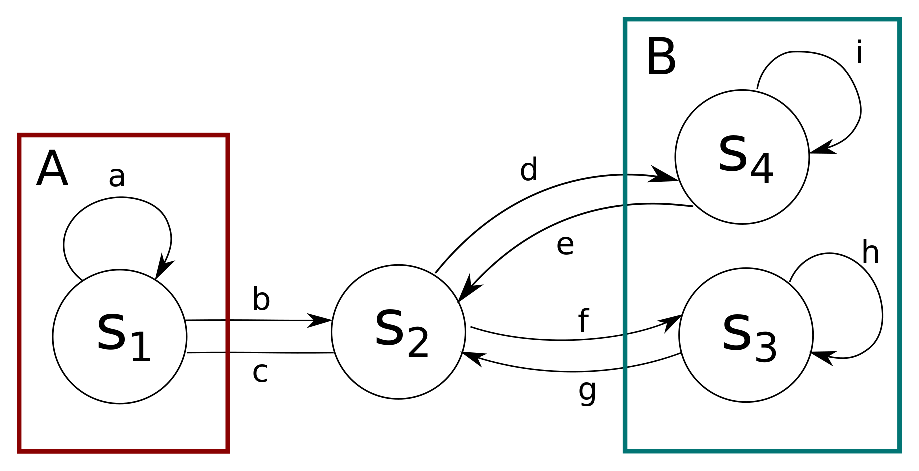
\includegraphics[width=0.4\linewidth]{pic/eg1}
	\caption{A simple AFTS with state space $\{s1,s2,s3,s4\}$ and action space $\{a,b,c, ...,h\}$, used to illustrate how the controller works. Atomic propositions are $ A =\{s_1\} $ and $ B=\{s_3, s_4\} $. For simplicity, assume no progress group exists.}  
	\label{fig:eg1}
\end{figure}

\begin{example}
	\label{ex:exec}
	For a simple AFTS shown in Figure \ref{fig:eg1}, given the specification $ \phi = \Square \Diamond A \wedge \Square \Diamond B $, the outputs of \eqref{win-phi} are the winning set $ W= \{s_1,s_2,s_3,s_4\}$, and the controller $ \mathcal{C} = (W,\{\mathcal{C}^0_1\}, x = 1) $, where its {\color{teal}descendant} controllers\footnote{In this example and  in Section \ref{sec:example}, a simple controller $ \mathcal{C}_{sim} $ is denoted by the set $ \{(s,\mathcal{C}_{sim}(s)): s\in D\} $ for simplicity, where $ D $ is the domain of $ \mathcal{C}_{sim} $.}
	 are:
	
	\noindent$ \mathcal{C}^0_1 = (\{W,\{s_1\},\{s_3,s_4\}\},\{\mathcal{C}^1_1, \mathcal{C}^1_2\}, x^0_1 ) $; 
	$ \mathcal{C}^1_1 = (\{\{s_1,s_2\},W,W \},\{\mathcal{C}^{2,0}_i\}_{i=1}^3,x^1_1)$; 
	
	\noindent$ \mathcal{C}^1_2 = (\{\{s_2,s_3,s_4\},W,W \},\{\mathcal{C}^{2,1}_i\}_{i=1}^{3},x^1_2 )$; $ \mathcal{C}^{2,0}_1 = \{(s_1,\{a\}),(s_2,\{c\})\} $; 
	
	\noindent$ \mathcal{C}^{2,0}_2 = \{(s_1,\{a,b\}),(s_2,\{c\}),(s_3,\{g\}),(s_4,\{e\})\} $;
	$ \mathcal{C}^{2,0}_3 = \{(s_1,\{a,b\}),(s_2,\{c,d,f\}),(s_3,\{g,h\}),(s_4,\{e,i\})\} $; 
	
	\noindent$ \mathcal{C}^{2,1}_1 = \{(s_2,\{d,f\}),(s_3,\{h\}),(s_4,i)\} $; $ \mathcal{C}^{2,1}_2 = \{(s_1,\{b\}),(s_2,\{d,f\}), (s_3,\{g,h\}), (s_4,\{e,i\})\} $;
	
	\noindent$ \mathcal{C}^{2,1}_3 = \{(s_1,\{a,b\}),(s_2,\{c,d,f\}),(s_3,\{g,h\}),(s_4,\{e,i\})\} $.
	
	\begin{figure}
		\centering
		\begin{subfigure}[b]{1\textwidth}
				\centering
				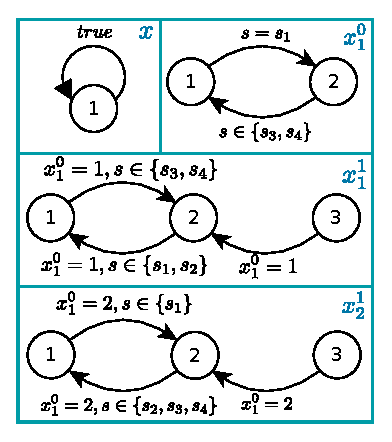
\includegraphics[width=0.85\linewidth]{pic/xupdate}
				\label{fig:xupdate1}
				\caption{no action disabled}
		\end{subfigure}
		\begin{subfigure}[b]{1\textwidth}
			\centering
			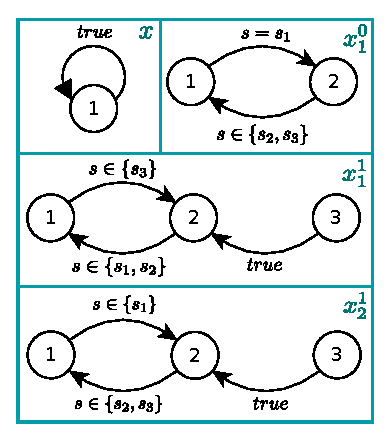
\includegraphics[width=0.85\linewidth]{pic/xupdate2}
			\label{fig:xupdate2}
			\caption{ action $ e $ is disabled}
		\end{subfigure}
		%\centering
		%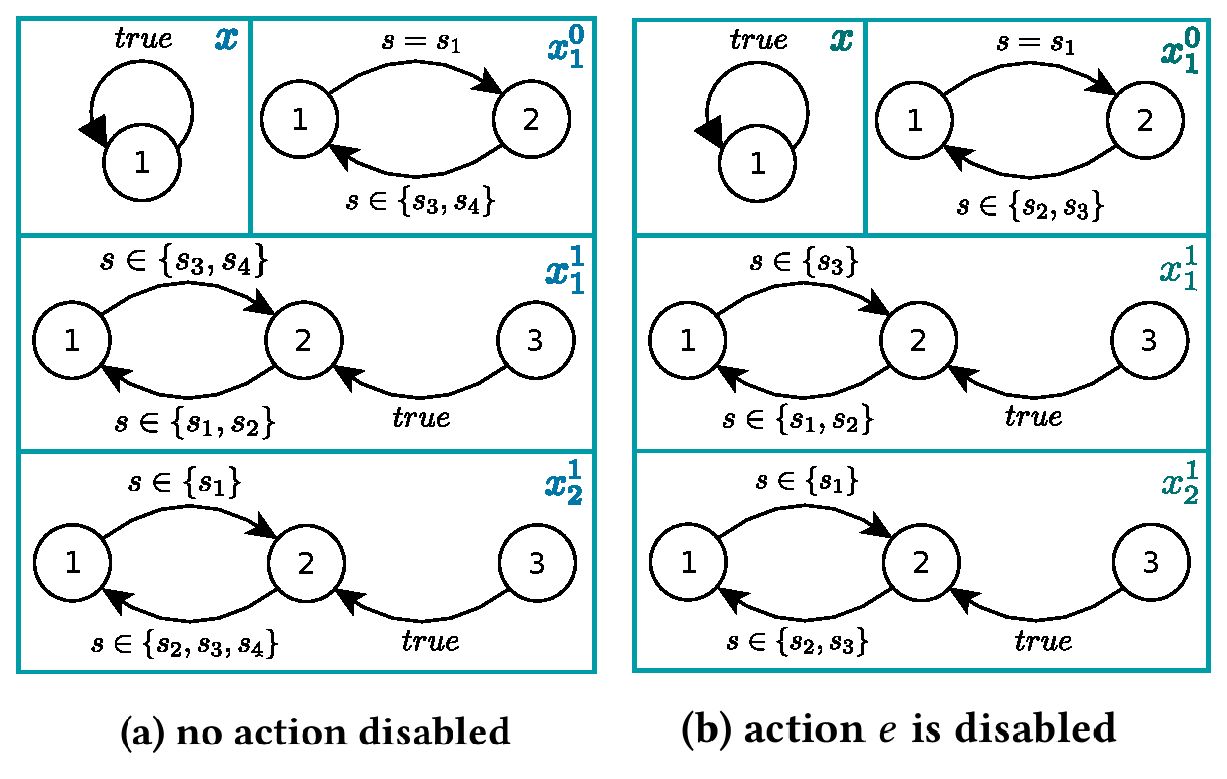
\includegraphics[width=0.8\linewidth]{pic/xupdate-full}
		\caption{ %{\color{purple} Same comment as on the previous version: it would be nice to see both transition graphs (before/after) side by side. Also: why do you show $x_1^0$ in the two bottom transitions; it could make the reader think that the transitions depend on the values of other internal variables, but it's not the case. The transition to children controllers is relatively clear to me, so I would simpy remove the value of other internal variables in each subgraph.}{\color{teal} the only change on the graph comes from changes in $ \mathcal{V} $ in each sub-controller.} 
            {\color{purple} I suggest to make the figures a bit wider.}
			The transition graph here is a visual illustration of the update rules of $ x $ in Definition \ref{def:exec}. (a) corresponds to the example \ref{ex:exec}. (b) corresponds to the example in Section \ref{sec:example1}. $s $ is the current state of the system in Figure \ref{fig:eg1}. At each execution time, each internal variable transits from its current node to one of the neighbor node once the transition condition on the edge is satisfied. If no transition condition is satisfied, internal variable remains unchanged. Update $ x$ first, and then $ x^0 $, and lastly $ x_0^1 $ and $x^1_1 $.} 
		\label{fig:xupdate}
	\end{figure}
	
	$ \mathcal{C} $, $ \mathcal{C}_1^0 $ and $ \mathcal{C}_i^1 $ result from \eqref{win-phi}, \eqref{win-interm} and \eqref{win-until}. $ \mathcal{C}_i^{2,k} $ are simple controllers resulting from \eqref{eqn:pre}. Each time $ \mathcal{C} $ is called, $ (x,x^0_1,x^1_1,x^1_2) $ is updated according to Definition \ref{def:exec}. The simple controllers in $ \mathcal{C} $ reached at that time determines the set of feasible control inputs. The update rules for internal variables in this example \ref{ex:exec} can be illustrated by the transition graph in Figure \ref{fig:xupdate}, which is consistent with Definition \ref{def:exec}. %is determined by $ \mathcal{C}^{2,k}_{x^1_{k}} (s)$ (if $ x^0 = k  $).
	
	For example, initialize the internal variables to be $ (1,1,1,1) $. Let's start from $ s_1 $ and run $ \mathcal{C}(s_1) $: The updated internal variables are $ (1,2,1,2) $, after $ \mathcal{C}(s_1), \mathcal{C}^0_1(s_1)$, $ \mathcal{C}^1_2(s_1) $ and $ \mathcal{C}^{2,1}_2(s_1) $ are called recursively. The set of feasible actions is $ \{b\}= \mathcal{C}^{2,1}_2(s_1) $. Under action $ b $, the system in Figure \ref{fig:eg1} transits to $ s_2 $. Now run $ \mathcal{C}(s_2) $. The internal variables are updated to $ (1,2,1,1) $. The set of feasible actions is $ \{d,f\}=\mathcal{C}^{2,1}_1(s_2) $. Let's keep doing this and always take the first action in the output of $ \mathcal{C} $ at each execution. The trajectory under control of $\mathcal{C} $ would be $ s_1,s_2,s_4,s_2,s_1,...$, where the sequence of actions is $ b,d,e,c,... $. The trajectory visits $ A $ and $ B $ in turn, satisfying the given specification.
	
	%\footnote{Define $ x_{total}: = (x,x^0,x^1_0,x^1_1) $. Each $ x_{total} $ locates a simple controller, i.g. $ x_{total}  = (0,1,0,5)$  gives that $ C_0^0\rightarrow C^1_1\rightarrow C^2_5 $. The evolution of $ x_{total} $ in the example above is $ (0,0,0,0), (0,1,0,5),(0,1,0,4), (0,0,1,4), (0,0,0,4)... $.}
\end{example}

%{\color{blue} don't use b.w., s,t, use between, such that. in general, it is better writing practice to avoid abbreviations as much as possible}

\subsection{Problem Statement}
\label{sec:prob}
In this section, we formally define the problem of interest. %{\color{blue}it is usually a good idea to start with telling what you want to do in the section so that the user is prepared.}

%{\color{purple} Somewhere we should give the main steps of the solution also. I think one thing that would be important is to state clearly what can and cannot change in the structure of the controller when $U$ is modified. I guess it is not only a change of the transitions, like in the example, since in some cases the number of steps to convergence can be modified. But then what exactly remains invariant? Only the "depth" of the controller? } {\color{teal} I think basically everything could be changed in the patching operator.} {\color{purple} OK}

\begin{problem}
	Given an AFTS $ T = (Q,U,\rightarrow_T,G,AP,h_Q) $, an LTL specification $ \phi = \Square A \wedge \Diamond \Square B \wedge \left( \bigvee_{i\in I} \Square \Diamond R^i\right) $, the winning set $ W_{\phi} $ and controller $ \mathcal{C}_{\phi} $, if a set of actions $ U_d\subseteq U $ in $ T $ is unavailable, find the new winning set and a controller with an algorithm that exploits the knowledge of $ W_{\phi} $ and $ \mathcal{C}_{\phi} $.\label{prob}
\end{problem}

We start by giving an overview of our solution approach. Recall that a controller in Definition \ref{def:cont} has a tree structure whose nodes consist of controllers (non-leaf nodes) and simple controllers (leaf nodes): the non-leaf nodes are computed by algorithm \eqref{win-interm}, \eqref{win-until} and \eqref{win-pgpre}; the leaf nodes are computed by algorithm \eqref{eqn:pre} and \eqref{win-inv} (see Appendix \ref{app:basic-alg}). Except for \eqref{win-phi}, each algorithm in the appendix corresponds to one underlying specification, specified by its input parameters. In Section \ref{sec:method}, we show that each algorithm in the appendix has a corresponding patching algorithm (denoted with an over-bar on the operator for the original algorithm) which restricts an existing controller resulting from it to a smaller action space for a stronger specification \footnote{In general, for specifications $ \phi $ and $ \psi $, ``$ \phi $ is stronger than $ \psi $"  means that whenever $ \phi $ is satisfied, $ \psi $ is satisfied. Here a stronger specification always refers to the case that the target set $ Z $ in the specification of a fixed-point based algorithm shrinks (if its specification has such a term, see Section \ref{sec:method}).}. These patching algorithms allow us to offer a solution to Problem \ref{prob} by patching the {\color{teal}descendant} controllers of a controller resulting from algorithm \eqref{win-phi} one by one. Furthermore, since there is an order between the nodes in each layer of the tree structure (recall that $ \mathcal{K} $ is a list), they need to be patched in the order that they are generated. 

To get the intuition, consider a simple invariance specification ($\Square A$) and the corresponding winning set $W_{\Square A}$ computed through a simple contracting fixed-point that starts with the set $A$ and shrinks this set until it finds the maximal invariant set that is contained in $A$. In this case the controller $\mathcal{C}_{\Square A}$ is just a chain (instead of an arbitrary tree) with a single simple controller. If the action set is reduced, then one can use the same simple contracting fixed-point with the new action set this time initialized with the set $W_{\Square A}$. Since $W_{\Square A}$ in general is smaller than $A$, the new fixed point algorithm needs less iterations. Our patching algorithm generalizes this idea to nested fixed-points where we systematically  restrict the inputs to each of the algorithms recursively, using the controller data structure introduced.  

%{\color{red}Also, for those nodes, their corresponding specifications, specified by the inputs of the algorithms generating them, need to be retrieved in order to figure out the invalid parts after changes in the action space. So to patch a controller resulting from a specific fixed-point based algorithm, we basically re-run that algorithm (so that we can easily retrieve the input parameters used for generating those node controllers), but replace the algorithms called internally to be their corresponding patching algorithms whose input parameters are the retrieved inputs, changes in the specification due to the disabled actions and the existing controller of that node. In this way, the correctness of that patching algorithm totally depends on the correctness of the patching algorithms it called internally. In the end, we show that as long as we can patch leaf nodes (simple controllers) and retrieve the original inputs for each fixed-point based algorithm correctly, the winning set corresponding to the modified controller is exactly the same as the winning set resulting from re-synthesizing a new controller.} 

\section{PATCHING METHOD}
\label{sec:method}

{\color{red} Not sure if this is still relevant: } %\sout{Before presenting the patching methods, we state a property of controller implementations that roughly shows that the controllers contain all the relevant information needed for patching. }
 Before presenting the patching methods, we state several properties of winning sets, which are vital to the success of patching existing controllers.

\iffalse
\begin{definition}
	For two control strategies $ \mu_1 $ and $ \mu_2 $
	%winning set $ W_1 $ and $ W_2 $
	 {\color{purple} over sets $D_1$ and $D_2$\footnote{In this work, $ D_1 $ and $ D_2 $ are always equal to the winning sets corresponding to $ \mu_1 $ and $ \mu_2 $. In general, they could be larger than the winning sets, depending on the type of specification.}}
	 	% (to avoid mentioning winning sets here)} ({\color{teal}a control strategy only takes inputs in the winning set, how to deal with this problem?})
  	 , we say that $ \mu_2 $ contains $ \mu_1$, denoted by $ \mu_{1} \subseteq \mu_{2}$, if $ \mu_{1} (\{(s_i,a_i)\}_{i=1}^{n-1}, s_n) $ is a subset of $ \mu_{2}(\{(s_i,a_i)\}_{i=1}^{n-1}, s_n) $, for all feasible $ n $ and all transition trajectories $ q =(s_1,a_1),(s_2,a_2),...,(s_{n-1},a_{n-1}) $ satisfying {\color{purple}$ s_1\in D_{1} $}, $ a_k \in \mu_{1} (\{(s_i,a_i)\}_{i=1}^{k-1}, s_k) $.
\end{definition}
\fi

Given an AFTS $ T = (Q,U,\rightarrow_T,G,AP,h_Q) $ and an LTL specification $ \phi $, compute its winning set $ W_{\phi} $ and the winning control strategy $ \mathcal{C}_{\phi} $  via the corresponding algorithm listed in Appendix \ref{app:basic-alg}. Now disable the set of actions $ U_d \subseteq U$ in the AFTS $ T $, which results in a new AFTS $ \widehat{T} = (Q,\widehat{U},\rightarrow_{\widehat{T}},G,AP,h_Q) $, where  $ \widehat{U} = U-U_d $ and $ \rightarrow_{\widehat{T}} = \rightarrow_T - \{(s_1,a,s_2):s_1,s_2\in Q, a\in U_d, (s_1,a,s_2)\in \rightarrow_T \} $. Re-compute the winning set and controller , denoted by $ \widehat{W}_{\phi} $ and $ \widehat{\mathcal{C}}_{\phi} $, for a specification the same as or stronger than $ \phi $ over $ \widehat{T} $ via the same algorithm. Here a stronger specification always refers that input parameter $ Z $ of algorithms \eqref{win-interm}, \eqref{win-pgpre}, \eqref{win-until} and  \eqref{win-inv} shrinks to a smaller set $ \widehat{Z}\subseteq Z $ (the other parameters are kept the same) after $ U_d $ is removed from the action space. Typically $ Z $ is the target set we want to reach, which shrinks due to the unavailable actions. 
Then, we have the following theorems, proofs of which are omitted for brevity:

\begin{theorem}
For algorithm \eqref{win-inv}, we have $ ( \widehat{W}_{\phi}\cup \widehat{Z}) \subseteq ( W_\phi \cup Z) $.\label{thm: inv-set}
\end{theorem}

%\emph{Proof:} $ W_\phi $ (resp. $ \widehat{W}_\phi $) resulting from algorithm \eqref{win-inv} is the largest subset of $ G\cap B-Z$ (resp. $ G\cap B -\widehat{Z} $) where $ B\  \mathbf{U}\ Z $ (resp. $ B\ \mathbf{U}\ \widehat{Z} $) can be enforced. It is easy to check that \eqref{win-inv} is sound and complete, i.e., the winning set contains all the feasible states and no spurious states. Because $ \widehat{Z} \subseteq Z $, $ B\mathbf{U} Z $ can be enforced for any state in $ \widehat{W}_\phi $. Thus by completeness, $ \widehat{W}_\phi - Z \subseteq W_\phi$. Furthermore, $ (\widehat{W}_\phi-Z) \cup Z = \widehat{W}_\phi \cup Z \subseteq W_\phi \cup Z$. For $ \widehat{Z}\subseteq Z $, $ \widehat{W}_\phi \cup \widehat{Z} \subseteq \widehat{W}_\phi \cup Z \subseteq  W_\phi \cup Z $. \QEDB

\begin{theorem}
For algorithms \eqref{win-phi}, \eqref{win-interm}, \eqref{win-until}, \eqref{win-pgpre} and \eqref{eqn:pre}, we have $ \widehat{W}_\phi \subseteq W_\phi $.

%	For $ W_{\phi}, \mu_{\phi}, \widehat{W}_{\phi}, \widehat{\mu}_{\phi} $ defined above, we have (i) $ \widehat{W}_{\phi} \subseteq W_{\phi} $ (ii) $ \widehat{\mu}_{\phi}\subseteq \mu_\phi $ if $ \mu_{\phi} $ and $ \widehat{\mu}_{\phi} $ are implemented by simple controllers. 
	\label{thm: 1} 
\end{theorem}

%\emph{Proof:} (a) For algorithms \eqref{win-phi}, \eqref{win-interm} and \eqref{win-until}: the winning sets are sound and complete, proven in \cite{Nilsson2017}. For any state $ s\in \widehat{W}_{\phi} $, if the system $ \widehat{T} $ starting from $ s $ could be controlled under an infinite sequence of actions and satisfy the specification $ \phi $, the same sequence of actions can be applied over $ T $ to get the same trajectory. Thus by completeness, $ s\in W_{\phi} $, and then $ \widehat{W}_{\phi}\subseteq W_{\phi} $. (b) For algorithm \eqref{win-pgpre}: Using Theorem \ref{thm: inv-set}, it can be easily proven by induction. (c) The case for \eqref{eqn:pre} is trivial. \QEDB

%Theorem \ref{thm: 1} says that the the domain of the existing controller always shrinks after a set of actions are disabled, which agrees with our intuition. Furthermore, it shows the containment relationship in simple controllers before and after changes in the action space, which reveals the possibility of patching the simple controllers instead of re-synthesizing them. 

If we fix the specification to be in the form of \eqref{phi}, Theorems \ref{thm: inv-set} and \ref{thm: 1} say that the winning sets of the controller and its nodes after $ U_d $ is disabled are bounded by winning sets of the controller and its nodes before $ U_d $ is disabled (or by the union of winning sets and $ Z $ for simpler controllers resulting from \eqref{win-inv}), which is the basis for our warm-starting synthesis method. Based on this fact, it's possible to search the feasible control strategies inside the existing controllers, i.e. patching the existing controllers, instead of re-synthesizing from scratch, for they contain the control strategies for a larger winning set than we need. Actually, we show that all the feasible control strategies for the new problem setting can be obtained by patching the existing controllers in the next two sections.

%In our context, controllers are the implementations of control strategies (see Definition \ref{def:cont}). If $ C_{\phi} $ is implemented to contain all the possible control strategies, Theorem \ref{thm: 1} says that {\color{teal}given the same sequence of inputs, the outputs of $ \widehat{\mathcal{C}}_{\phi} $ should be contained by the outputs of $ \mathcal{C}_{\phi} $}, which implies there is a possibility to obtain $ \widehat{\mathcal{C}}_{\phi} $ by patching the existing controller $ \mathcal{C}_{\phi} $. %{\color{purple} I have mixed feeling about this last remark; "contain all the information" is a vague notion}


%From the perspective of implementation, a controller $ \mathcal{C}=(\mathcal{V},\mathcal{K},x) $ is a data structure that organizes simple controllers in a hierarchy way. The partially ordered sets $ \mathcal{V} $  and internal variable are only used during execution. So the basic step for patching a controller is to modify its simple controllers, which are discussed in Section \ref{sec:patch-simple}. 


\subsection{Patching Simple Controllers}
\label{sec:patch-simple}
A controller is a tree structure built on simple controllers, i.e. the leaf nodes in the tree structure. Thus we need to patch the leaf nodes firstly, and then patch their parent nodes, and so forth.  In this section, we discuss the patching algorithms for the simple controllers, and then in the following section we will show how to patch the other nodes building on the leaf nodes, and the controller resulting from \eqref{win-phi}. 

\begin{definition}
	Given a simple controller $ \mathcal{C} $ over an AFTS $T = (Q,U,\rightarrow_T, G,AP,h_Q) $, a \textbf{finite transition system} (FTS) corresponding to $ \mathcal{C} $ is $A(\mathcal{C}) = (Q_C, U_C, \rightarrow_{A(\mathcal{C})})$ %{\color{purple} I'm not sure $T(C)$ is the best notation, since $T$ is usually our AFTS; A(C)?}
	, where $ Q_C $ is the set of states that appear in $ \rightarrow_{A(\mathcal{C})} $, $ U_C=\{u: u\in \mathcal{C}(s), \forall s\in D\} $, $ \rightarrow_{A(\mathcal{C})} =\{(s_1,u,s_2)\in \rightarrow_T: s_1\in D,s_2\in Q, u\in \mathcal{C}(s_1)\} ${\color{teal}, and $ D $ is the domain of $ \mathcal{C} $}. \label{def:TC}
\end{definition}

\begin{remark}
	By Definition \ref{def:TC}, $ A(\mathcal{C}) $ can be easily constructed from the simple controller $ \mathcal{C} $ and the AFTS $ T $. Conversely, $ \mathcal{C} $ can be constructed from $ A(\mathcal{C}) $ by $ \mathcal{C} = \{(s,D(s)):s\in W,D(s)\not=\emptyset\} $, where $ D(s)=\{u:(s,u,s_2)\in \rightarrow_{A(\mathcal{C})}\} $.\label{rmk:conv}
\end{remark}
%{\color{blue} don't abbreviate "not", write "do not", "does not", etc.}
{\color{teal} $ A(\mathcal{C}) $ contains the transitions behind the state-action pairs in $ \mathcal{C} $, so that we can search invalid transitions in $ A(\mathcal{C}) $ after some actions become unavailable. Also, by Remark \ref{rmk:conv}, it's easy to transfer between  $ \mathcal{C} $ and $ A(\mathcal{C}) $.} Therefore, we patch a simple controller $ \mathcal{C} $ by modifying its corresponding FTS $ A(\mathcal{C}) $ and then transferring $ A(\mathcal{C}) $ to $ \mathcal{C} $. Several operations applied to the FTS $ A(\mathcal{C}) $ are defined in Table \ref{tab:oper}, with which we are ready to modify simple controllers resulting from \eqref{eqn:pre} and \eqref{win-inv}, i.e. $ \text{Pre}_{\exists,\forall}^{T, U}(V) $ and $ \text{Inv}_{\exists}^{D,G}(Z,B) $. %{\color{purple} Not clear}

%Assume the AFTS $ T = (Q,U,\rightarrow_T, G, AP, h_Q) $ is the abstraction of the system that needs to be controlled. Assume that $ A(\mathcal{C})=(Q_{\mathcal{C}}, U_{\mathcal{C}},\rightarrow_{A(\mathcal{C})})$ is a transition system corresponding to a simple controller $ \mathcal{C} $. 

%Firstly let's define several operation to manipulate the finite transition system $ A(\mathcal{C}) $:

%\emph{transitions removing}: given $ E = \{(s_1,a,s_2): s_1,s_2\in Q_{\mathcal{C}}, a\in U_{\mathcal{C}}\} $, remove all transitions in $ E $ from $ A(\mathcal{C}) $ i.e. replace $ \rightarrow_{A(\mathcal{C})} $ with $\rightarrow_{A(\mathcal{C})} - E$, written as 
%\begin{displaymath}
%	A(\mathcal{C})\backslash E 
%\end{displaymath}

%\emph{transition adding}: given $ E \subseteq Q \times U \times Q$, replace $ \rightarrow_{A(\mathcal{C})} $ with $ \rightarrow_{A(\mathcal{C})}\cup E $, denoted for simplicity by
%\begin{displaymath}
%A(\mathcal{C})\cup E
%\end{displaymath}

%Note that since $ E \subseteq Q\times U\times Q $, $ E $ may contain states and actions which do not exists in $ Q_{\mathcal{C}}\subseteq Q $ and $ U_{\mathcal{C}}\subseteq U $. Then just assume that $ Q_{\mathcal{C}} $ and $ U_{\mathcal{C}} $ will enlarge automatically, which is easy to implement in the code.

%\emph{null node seeking}: return the set $\{s_1\in Q_{A(\mathcal{C})}: \not\exists (s_1,a,s_2)\in \rightarrow_{A(\mathcal{C})},\forall a\in U_{A(\mathcal{C})}, \forall s_2 \in Q_{A(\mathcal{C})}\} $, i.e. all the nodes whose out-degree is zero, written as
%\begin{displaymath}
%Vac(A(\mathcal{C}))
%\end{displaymath}

%\emph{state-action pre}: return the set $ \{(s_1,a): (s_1,a,s_2)\in \rightarrow_{A(\mathcal{C})}, s_2\in S_2\} $, i.e. all the edges pointing into nodes in $ S_2 $, written as
%\begin{displaymath}
%\widehat{Pre}^{A(\mathcal{C}),U}_{\exists,\exists}(S_2)
%\end{displaymath}

\begin{table*}
	\centering
	\caption{Basic Operations on the FTS corresponding to controller $ \mathcal{C} $}
	\begin{tabular}{ccc}
		\hline
		Operation & Definition & Notation\\
		\hline
		\emph{transition removing} & given $ E\subseteq Q\times U\times Q $, replace $ \rightarrow_{A(\mathcal{C})} $ with $\rightarrow_{A(\mathcal{C})} - E$ & $ A(\mathcal{C})\backslash E $\\
		\emph{transition adding} & given $ E\subseteq Q\times U\times Q $, replace $ \rightarrow_{A(\mathcal{C})} $ with $ \rightarrow_{A(\mathcal{C})}\cup E $ & $ A(\mathcal{C})\cup E $\\
		\emph{state-action pre} &  Given $ S_2\subseteq Q $, output $ \{(s_1,a): (s_1,a,s_2)\in \rightarrow_{A(\mathcal{C})}, s_2\in S_2\} $ & $ \widehat{Pre}^{A(\mathcal{C}),U}_{\exists,\exists}(S_2) $\\
		\hline
	\end{tabular}
	\label{tab:oper}
\end{table*}

{\color{red}being an abstraction is not really relevant I think} 
Suppose that  $ W $ and $ \mathcal{C} $ are the winning set and controller resulting from $ \text{Pre}_{\exists,\forall}^{T, U}(V) $. Given $ \widehat{V}= V-\Delta V $ {\color{teal}\sout{and $ \widehat{U} = U-U_d $}}, we want to modify $ W $ and $ \mathcal{C} $ to be the winning set and controller resulting from $ \text{Pre}_{\exists,\forall}^{\widehat{T},\widehat{U}}(\widehat{V}) $. Intuitively if we can find all the invalid transitions $ (s_1,u,s_2) $ in $ A(\mathcal{C}) $ due to $ u\in U_d $ or $ s_2\in\Delta V $, and remove them from $ A(\mathcal{C}) $, that would result in a controller that works for the new problem setting, based on which, the patching operator for \eqref{eqn:pre} is:
{\small
\begin{align}
&[\widehat{W},\widehat{\mathcal{C}}]=\overline{\text{Pre}}_{\exists,\forall}^{T, U}(\mathcal{C},\Delta V,U_d)\nonumber\\
=&\begin{cases} 
T_{0} = A(\mathcal{C})\backslash (*,U_d,*)\\
E =  \widehat{Pre}^{T_0,U-U_d}_{\exists,\exists}(\Delta V)\\
A(\widehat{\mathcal{C}}) = T_{0}\backslash E\\
\widehat{W} = \{s_1: \exists u, \exists s_2 s.t. (s_1,u, s_2)\in \rightarrow_{A(\widehat{\mathcal{C}})} \}
\end{cases}\label{patch-pre}
\end{align}}
where $ \widehat{\mathcal{C}} $ is converted from $ A(\widehat{\mathcal{C}}) $. $ \widehat{W} $ and $ \widehat{\mathcal{C}} $ are the modified winning set and controller.

\begin{theorem}
	$ \widehat{W} $ and $ \widehat{\mathcal{C}} $ returned by \eqref{patch-pre} are the same as the outputs resulting from $ \text{Pre}_{\exists,\forall}^{\widehat{T},\widehat{U}}(\widehat{V})$ in \eqref{eqn:pre}.	\label{thm:pre}
\end{theorem}

\emph{Proof:} Suppose that $ \text{Pre}_{\exists,\forall}^{\widehat{T},\widehat{U}}(\widehat{V}) $ returns $ W_t $ and $ \mathcal{C}_t $. It's enough to show that $ A(\widehat{\mathcal{C}})= A(\mathcal{C}_t)$, i.e. $ \rightarrow_{A(\widehat{\mathcal{C}})} = \rightarrow_{A(\mathcal{C}_t)} $. By \eqref{eqn:pre} and Definition \ref{def:TC}, it is obvious that $ \rightarrow_{A(\mathcal{C}_t)} \subseteq \rightarrow_{A(\mathcal{C})}$ for $ \widehat{V}\subseteq V $ and $ \widehat{U}\subseteq U $. The set of transitions $ S = (*,U_d,*)\cup E $ is only related to states in $ \Delta V $ or actions in $ U_d $, so $\rightarrow_{A(\mathcal{C}_t)}$ and $ S $ are disjoint. $ \rightarrow_{A(\widehat{\mathcal{C}})}= \rightarrow_{A(\mathcal{C})}-S$. Thus $ \rightarrow_{A(\mathcal{C}_t)}\subseteq \rightarrow_{A(\widehat{\mathcal{C}})}$. By \eqref{patch-pre}, transitions in $ A(\widehat{\mathcal{C}}) $ can only take actions in $ \widehat{U} $ and transit to states in $ \widehat{V} $, which implies that $ \rightarrow_{A(\widehat{\mathcal{C}})}\subseteq \rightarrow_{A(\mathcal{C}_t)} $. \QEDB 


Suppose that $ Y $ and $ \mathcal{C} $ are the winning set and controller resulting from $ \text{Inv}_{\exists}^{D,G}(Z,B) ${\color{teal}\sout{, and $ U_d $ is a set of actions unavailable}}. If $ D\cap U_d \not= \emptyset$, the winning set is empty by the definition of progress group (see\cite{Nilsson2017}). Given $ \widehat{Z} \subseteq Z $ and $D$ such that $ D\cap U_d=\emptyset $, we want to modify $ Y $ and $ \mathcal{C} $ to be the winning set and controller for $ \text{Inv}_{\exists}^{D,G}(\widehat{Z}, B) $.  The modified winning set $\widehat{Y}$ is contained by $ Y\cup (\Delta Z\cap G\cap B) $. Also, $ \text{Inv}_{\exists}^{D,G}(Z,B) $ computation in \eqref{win-inv} is a contraction algorithm in the sense that $ \{Y_k\}_{k=1}^{\infty} $ is a monotonic decreasing sequence whose limit is the winning set. Combining these two facts, we can warm-start the contraction algorithm in \eqref{win-inv} with $ Y_0=Y\cup (\Delta Z\cap G\cap B)$ instead of $ Q $. The patching operator is
{\small\begin{align}
&[\widehat{Y},\widehat{\mathcal{C}}]=\overline{Inv}_{\exists}^{D,G}(Y,\mathcal{C},Z,\widehat{Z})\nonumber \\
=&\begin{cases}
Y_0 = Y\cup (\Delta Z\cap G \cap B)\\
\Delta Y_0 = Q - (Y_0 \cup \widehat{Z})\\
T_0  = A(\mathcal{C})\cup E_0\\
{\color{black} k=0}\\
%while \ Y_{k+1}\not= Y_k:\\
{\color{black} repeat:}\\
\end{cases}
\begin{cases}
\ \ \ \ \Delta Y_{k+1} = \Delta Y_k \cup \text{Pre}_{\forall,\exists}^{T_k,D}(\Delta Y_k) \\
\ \ \ \ T_{k+1} = T_{k}\backslash (\Delta Y_{k+1},*,*)\\
\ \ \ \ Y_{k+1} = Y_k- \Delta Y_{k+1}\\
\ \ \ \ {\color{black} k=k+1}\\
{\color{black} until \ Y_k = Y_{k-1}}\\
\widehat{Y}=Y_k,\ A(\widehat{\mathcal{C}}) = T_{k}
\end{cases}\label{patch-inv}
\end{align}}
where $ \Delta Z = Z - \widehat{Z} $, $ E_0 = \{(s_1,a,s_2)\in \rightarrow_{T}: s_1\in Y_0, a\in D, s_2 \in Q\} $, $ \text{Pre}_{\forall,\exists}^{T_k,D}(\Delta Y_k) = \{q_1: \forall u\in D, \exists q_2\in \Delta Y_k, s.t.\ (q_1, u, q_2) \in \rightarrow_{T_k} \} $. $ \widehat{Y} $ is the modified winning set, and the controller $ \widehat{\mathcal{C}} $ can be recovered from $ A(\widehat{\mathcal{C}}) $.

In regards to the patching operator in \eqref{patch-inv}, we have the following result, proof of which is given in Appendix \ref{app:pr-31}:

\begin{theorem}
	$ \widehat{Y} $ and $ \widehat{\mathcal{C}} $ returned by \eqref{patch-inv} are the same as the outputs resulting from $ \text{Inv}_{\exists}^{D,G}(\widehat{Z},B) $ in \eqref{win-inv}.	\label{thm:inv}
\end{theorem}
Given a simple controller $ \mathcal{C} $ and new synthesis settings, both \eqref{patch-pre} and \eqref{patch-inv} try to find $ A(\widehat{\mathcal{C}}) $ inside $ A(\mathcal{C}) $. However, if we re-synthesize the new simple controller from scratch, \eqref{eqn:pre} and \eqref{win-inv} would try to find $ A(\mathcal{C}) $ in the whole AFTS $ T $, which in general needs more computation cost, demonstrated by the simulation results in Section \ref{sec:example}. However, in the worst case, there might not be any computational gains.

\subsection{Patching General Controllers}
\label{sec:patch-cont}
%\begin{assumption}
%	A fixed-point patching operators has access to outputs and inputs of the corresponding fixed-point operator, as well as all the intermediate winning sets and controllers of the fixed-point operators generated at each iterative step. 
%\end{assumption}

In the section we are going to patch all the non-leaf nodes, i.e  the controllers resulting from \eqref{win-interm}, \eqref{win-until}, \eqref{win-pgpre}, and the root node, i.e. the controller result from \eqref{win-phi}, and finally Theorem \ref{thm:phi} shows that the patching algorithm for \eqref{win-phi} offers a solution to the Problem \ref{prob} in Section \ref{sec:prob}.

%The basic idea behind the patching algorithms are the same: All the fixed-point operators considered in this section are either expanding algorithms  (\eqref{win-phi}, \eqref{win-until},\eqref{win-pgpre}) or contraction algorithm \eqref{win-interm} in the sense that $ \{W_k\}_{k=0}^\infty $ (or $ Z_k, X_k,V_k $ depending on  which fixed-point operator we consider) is a monotonic sequence in $ 2^Q $ whose limit is the winning set. Also, it is easy to see that the modified winning set would be contained by the original one. Motivated by those facts, our patching algorithm warm-starts the expanding or contraction process in the original algorithm based on patching the existing winning sets and controllers.


Assume that $ Z $ and $ \mathcal{C} = (\mathcal{V},\mathcal{K},x) $ are the winning set and controller resulting from  $ \text{PGPre}_{\exists,\forall}^{T} (Z,B)$. Given $ \widehat{Z}\subseteq Z ${\color{teal}\sout{,  $ \widehat{U}\subseteq U $}}, we want to modify $ Z $ and $ \mathcal{C} $ to be the winning set and controller for $ \text{PGPre}_{\exists, \forall}^{\widehat{T}}(\widehat{Z},B)$. The patching operator is:
{\small\begin{align}
\begin{split}
&[\widehat{Z}_{\infty},\widehat{\mathcal{C}}]=\overline{\text{PGPre}}_{\exists,\forall}^{T} (\mathcal{C},Z,\widehat{Z},U_d)\\
&= \begin{cases}
Z_{\infty} = Z,\ \widehat{Z}_{\infty}=\widehat{Z},\ \widehat{\mathcal{V}}=\{\},\ \widehat{\mathcal{K}}=\{\},\ k = 1\\
for\ D\in 2^U:\\
\ \ for\ G\in G(D):\\
\ \ \ \ \ \ if\ U_d\cap D = \emptyset:\\
\ \ \ \ \ \ \ \ \  [\widehat{\mathcal{V}}(k),\widehat{\mathcal{K}}(k)]=\overline{Inv}_{\exists}^{D,G}(\mathcal{V}(k),\mathcal{K}(k),Z_\infty, \widehat{Z}_\infty)\\
\end{cases}
\begin{cases}
\ \ \ \ \ \ else:\ \widehat{\mathcal{V}}(k)=\emptyset, \widehat{\mathcal{K}}(k) = \emptyset\\
\ \ \ \ \ \  Z_\infty = Z_\infty\cup \mathcal{V}(k),\ \widehat{Z}_{\infty} = \widehat{Z}_{\infty} \cup \widehat{\mathcal{V}}(k)\\
\ \ \ \ \ \ {\color{black} k = k+1}\\
Remove\ all\ \emptyset\ in\ \widehat{\mathcal{V}}\ and \ \widehat{\mathcal{K}},\ \ 
\widehat{\mathcal{C}} = (\widehat{\mathcal{V}},\widehat{\mathcal{K}},x)
\end{cases}\label{patch-pg}
\end{split}
\end{align}}

\begin{theorem}
	$ \widehat{Z}_\infty $ and $ \widehat{\mathcal{C}} $ returned by \eqref{patch-pg} are the same as outputs resulting from $ \text{PGPre}_{\exists, \forall}^{\widehat{T}}(\widehat{Z},B)$ in \eqref{win-pgpre}.	\label{thm:pg}
\end{theorem}

\emph{Proof:} By theorem \ref{thm:inv}, the results of \eqref{patch-pg} remain the same if we replace $ \overline{Inv}_{\exists}^{D,G}(\mathcal{V}(k),\mathcal{K}(k),Z_\infty, \widehat{Z}_\infty)$ in \eqref{patch-pg} with $ Inv_\exists^{D,G}(\widehat{Z}_{\infty}) $. After the replacement, the algorithm \eqref{patch-pg} is the same as the algorithm \eqref{win-pgpre}. Therefore, their outputs must be the same. \QEDB


Assume that $ X_\infty $ and $ \mathcal{C}=(\mathcal{V},\mathcal{K},x) $ are the winning set and controller resulting from $ \text{Win}_{\exists,\forall}^{T}(B\mathbf{\ U\ }Z) $. Assume $ \vert \mathcal{K}\vert = 2n $, i.e. \eqref{win-until} converges in $ n $ steps. Then, given $ \widehat{Z}\subseteq Z ${\color{teal} \sout{and $ \widehat{U}= U-U_d $}}, to get the winning set and controller for $ \text{Win}_{\exists,\forall}^{\widehat{T}}(B\mathbf{\ U\ }\widehat{Z}) $, the patching operator is
{\small\begin{align}
\begin{split}
&[\widehat{X}_\infty, \widehat{\mathcal{C}}]=\overline{\text{Win}}^{T}_{\exists,\forall, (B\mathbf{\ U\ }Z)}(\mathcal{C},Z,\widehat{Z}, U_d)\\
=&\begin{cases}
X_0 = \emptyset, \widehat{X}_0 = \emptyset, \Delta X = \emptyset, \ \widehat{\mathcal{V}}=\{\},\ \widehat{\mathcal{K}}=\{\}\\
%{\color{purple} remove: } for ~ k\in \{0,2,...,n-1\}\ and\ \widehat{X}_{k+1}\not=\widehat{X}_k:\\
{\color{black} k = 0}\\
{\color{black} repeat:}\\
\ \ \ \ [\widehat{\mathcal{V}}(2k+1),\widehat{\mathcal{K}}(2k+1)] =\\ \ \ \ \ \ \ \ \ \  \overline{\text{Pre}}_{\exists,\forall}^{T,U}(\mathcal{K}(2k+1),X_{k}-\widehat{X}_{k}, U_d)\\
\ \ \ \ E_k = Z\cup (B\cap \mathcal{V}(2k+1))\\
\ \ \ \  \widehat{E}_k =  Z\cup (B\cap \widehat{\mathcal{V}}(2k+1))\\
\ \ \ \ [\widehat{\mathcal{V}}(2k+2),\widehat{\mathcal{K}}(2k+2)] =\\ \ \ \ \ \ \ \ \ \  \overline{\text{PGPre}}_{\exists,\forall}^{T}(\mathcal{K}(2k+2),E_k, \widehat{E}_k,U_d)\\ 
\ \ \ \ X_{k+1} = Z\cup (B\cap \mathcal{V}(2k+1)) \cup \mathcal{V}(2k+2)\\
\ \ \ \ \widehat{X}_{k+1} =\widehat{Z}\cup (B\cap \widehat{\mathcal{V}}(2k+1)) \cup \widehat{\mathcal{V}}(2k+2)\\
\end{cases}
\begin{cases}
\ \ \ \ {\color{black} k = k +1}\\
{\color{black} until \ k = n \ or \ \widehat{X}_{k}=\widehat{X}_{k-1}}\\
%{\color{purple} remove: }for~k\geq n\ and\ \widehat{X}_{k+1}\not=\widehat{X}_k:	\\
{\color{black} while \ \widehat{X}_{k}\not=\widehat{X}_{k-1}:}\\
\ \ \ \ [\widehat{\mathcal{V}}(2k+1),\widehat{\mathcal{K}}(2k+1)] = \\ \ \ \ \ \ \ \ \ \overline{\text{Pre}}_{\exists,\forall}^{T,U}(\mathcal{K}(2n-1),X_{n}-\widehat{X}_{k}, U_d)\\
\ \ \ \ \widehat{E}_k =  Z\cup (B\cap \widehat{\mathcal{V}}(2k+1))\\
\ \ \ \ [\widehat{\mathcal{V}}(2k+2),\widehat{\mathcal{K}}(2k+2)] =\\ 
\ \ \ \ \ \ \ \ \overline{\text{PGPre}}_{\exists,\forall}^{T}(\mathcal{K}(2n),E_n, \widehat{E}_k,U_d)\\
\ \ \ \ \widehat{X}_{k+1} =\widehat{Z}\cup (B\cap \widehat{\mathcal{V}}(2k+1)) \cup \widehat{\mathcal{V}}(2k+2)\\
\ \ \ \ {\color{black} k=k+1}\\
\widehat{X}_\infty = \widehat{X}_k,\ \widehat{\mathcal{C}} = (\widehat{\mathcal{V}},\widehat{\mathcal{K}},x)
\end{cases} \label{patch-until}
\end{split}
\end{align}}

In the algorithm \eqref{patch-until}, for $ k <n $, we patch the $ (2k+1) $th and $ (2k+2) $th existing sub-controllers in $ \mathcal{K} $. If the winning set doesn't converge in $ n $ iterations, for $ k\geq n $, we duplicate the last two existing sub-controllers to the tail of $ \mathcal{K} $, and patch them to enlarge the winning set until convergence. 
\begin{theorem}
	$ \widehat{X}_\infty $ and $ \widehat{\mathcal{C}} $ returned by \eqref{patch-until} are the same as outputs resulting from $ \text{Win}_{\exists,\forall}^{\widehat{T}}(B\mathbf{\ U\ }\widehat{Z})  $ in \eqref{win-until}.\label{thm:until}	
\end{theorem}

\emph{Proof:} Similar to the proof of Theorem \ref{thm:pg}, we can replace all the $ \overline{Pre}_{\exists,\forall}^{T,U} $ and $ \overline{PGPre}_{\exists,\forall}^{T} $ terms with $ \overline{Pre}_{\exists,\forall}^{\widehat{T},\widehat{U}}(\widehat{X}_k) $ and $PGPre_{\exists,\forall}^{\widehat{T}}(\widehat{E_k},B)$. Theorem \ref{thm:pre} and \ref{thm:pg} guarantee that the replacements are equivalent, but we need to verify: (i) $ \widehat{X}_k \subseteq X_k $ and $ \widehat{E}_k \subseteq E_k $ for $ k < n $, and (ii) $ \widehat{X}_k \subseteq X_n $ and $ \widehat{E}_k \subseteq E_n $ for $ k\geq n $. Both (i) and (ii) can be easily checked using induction argument and Theorem \ref{thm: 1} ( base case: $ \widehat{X}_0\subseteq X_0 $ and $ \widehat{E}_1\subseteq E_1 $). After the equivalent replacements, algorithm \eqref{patch-until} and algorithm \eqref{win-until} become the same. Thus their outputs must be the same. \QEDB

Assume that $ W $ and $ \mathcal{C}=(\mathcal{V},\mathcal{K},x) $ are the winning set and controller resulting from $\text{Win}_{\exists,\forall}^{T}((B\mathbf{\ U\ }Z)\vee \Square(B\wedge (\bigwedge_{i\in I} \Diamond R^i)) $. Given that $ \widehat{Z}\subseteq Z $ and $ \widehat{U}\subseteq U $, patch $ W $ and $ \mathcal{C} $ for $\text{Win}_{\exists,\forall}^{T}((B\mathbf{\ U\ }\widehat{Z})\vee \Square(B\wedge (\bigwedge_{i\in I} \Diamond R^i)) $. The patching operator for \eqref{win-interm} is 
{\small\begin{align}
&[\widehat{W}_{\infty},\widehat{\mathcal{C}}]=\overline{\text{Win}}^{T}_{\exists,\forall (\psi)} (\mathcal{C},Z,\widehat{Z},U_d)\nonumber\\
=&\begin{cases}
W_0 = \mathcal{V}(1),\widehat{\mathcal{V}}=\mathcal{V},\widehat{\mathcal{K}}=\mathcal{K}\\
Z_{\infty}^i = Z\cup (B\cap R^i\cap \text{Pre}_{\exists, \forall}^{T,U}(W_0))\\
\widehat{Z}_{0}^i = \widehat{Z}\cup (B\cap R^i\cap \text{Pre}_{\exists, \forall}^{T,U-U_d}(W_0))\\
[X^i_0,\widehat{\mathcal{K}}(i)] = \overline{\text{Win}}^{T}_{\exists,\forall, (B\mathbf{U}Z)}(\widehat{\mathcal{K}}(i),Z_\infty^i,\widehat{Z}_0^i, U_d)\\
\widehat{W}_{0} = \bigcap_{i\in I} X^i_0\\
{\color{black} k=0}
\end{cases}
\begin{cases}
%{\color{black} remove:} while\ \widehat{W}_{k+1}\not=\widehat{W}_k:\\
{\color{black} repeat:}\\
\ \ \ \ \widehat{Z}_{k+1}^i = \widehat{Z} \cup (B\cap R^i\cap \text{Pre}_{\exists, \forall}^{T,U-U_d}(\widehat{W}_k))\\
\ \ \ \ [X^i_{k+1},\widehat{\mathcal{K}}(i)]=\overline{\text{Win}}^{T}_{\exists,\forall,(B\mathbf{U}Z)}(\widehat{\mathcal{K}}(i),\widehat{Z}_k^i,\widehat{Z}_{k+1}^i, U_d)\\
\ \ \ \ \widehat{W}_{k+1} = \bigcap_{i\in I} X^i_{k+1}\\
\ \ \ \ {\color{black} k = k+1}\\
{\color{black} until \ \widehat{W}_{k}=\widehat{W}_{k-1}}\\
\widehat{W}_\infty = \widehat{W}_k,\ \widehat{\mathcal{C}}=(\widehat{\mathcal{V}},\widehat{\mathcal{K}},x)
\end{cases}\label{patch-interm}
\end{align}
}
\begin{theorem}
	$ \widehat{W}_\infty $ and $ \widehat{\mathcal{C}} $ returned by \eqref{patch-until} are the same as outputs resulting from $\text{Win}_{\exists,\forall}^{\widehat{T}}((B\mathbf{\ U\ }\widehat{Z})\vee \Square(B\wedge (\bigwedge_{i\in I} \Diamond R^i)) $ in \eqref{win-interm}. \label{thm:interm}	
\end{theorem}
\emph{Proof:} Assume that $ W_t $ is the winning set resulting from $\text{Win}_{\exists,\forall}^{\widehat{T}}((B\mathbf{\ U\ }\widehat{Z})\vee \Square(B\wedge (\bigwedge_{i\in I} \Diamond R^i)) $. Similar to the proof of Theorem \ref{thm:until}, we can replace all the $ \overline{Win}^{T}_{\exists,\forall} $ terms in \eqref{patch-interm} with $ Win^{\widehat{T}}_{\exists,\forall}(B\mathbf{U}\widehat{Z}_k^i) $, as long as (i) $ \widehat{Z}_0^i\subseteq Z_\infty^i $ and (ii) $ \widehat{Z}_{k+1} \subseteq \widehat{Z}_{k} $ are true. (i) is trivial. For (ii), it's enough to show that $ \widehat{W}_{k+1}\subseteq \widehat{W}_k $, which can be proven by induction. The base case: Since (i) is true, by Theorem \ref{thm:until}, we have $ X_0^i = Win_{\exists,\forall}^{\widehat{T}}(B\mathbf{U}\widehat{Z}) $. Then $ \widehat{W}_0 =\bigcap_{i\in I} \text{Win}_{\exists,\forall}^{\widehat{T}}(B\mathbf{\ U\ }\widehat{Z}_0^i)\subseteq \bigcap_{i\in I} \text{Win}_{\exists,\forall}^{T}(B\mathbf{\ U\ }Z_{\infty}^i) = W_0 $ by Theorem \ref{thm: 1}. Assume that $ \widehat{W}_{k+1} \subseteq \widehat{W}_k $.  Then $ \widehat{Z}_{k+1}^i\subseteq \widehat{Z}_{k}^i  $ and $ \widehat{W}_{k+1} =\bigcap_{i\in I} \text{Win}_{\exists,\forall}^{\widehat{T}}(B\mathbf{\ U\ }\widehat{Z}_{k+1}^i)\subseteq \bigcap_{i\in I} \text{Win}_{\exists,\forall}^{T}(B\mathbf{\ U\ }\widehat{Z}_{k}^i) = \widehat{W}_k $. Therefore by induction argument $ \widehat{W}_{k+1}\subseteq \widehat{W}_k $, and $ \widehat{Z}_{k+1}\subseteq \widehat{Z}_k $ for all $ k $. Then (ii) is true. After the replacements, \eqref{patch-interm} and \eqref{win-interm} are the same except that the contraction of $ W_k $ starts from the existing winning set $ W $ instead of $ Q $. We can show that $ W_t \subseteq \widehat{W}_k $ for all $ k $ by induction (base case: $ W_t \subseteq W_0$ by Theorem \ref{thm: 1}). Also $ W_t $ is the largest fixed point in $ Q $ by definition. So both \eqref{patch-interm} and \eqref{win-interm} will converge to the same fixed point $ W_t$.  \QEDB

Finally we are ready to patch the controller resulting from \eqref{win-phi} for specification in the form of \eqref{phi}.

Assume that $ W $ and $ \mathcal{C}=(\mathcal{V},\mathcal{K},x) $ are the winning set and controller resulting from the operator $
\text{Win}_{\exists, \forall}^{T}\left(\Square A \wedge \Diamond \Square B \wedge \left( \bigwedge_{i\in I} \Square \Diamond R^i\right)\right)$. Assuming that $ \vert \mathcal{K}\vert = n $. For patching purpose, we need some extra information: the lists of winning sets and controllers returned by $\text{Pre}_{\exists,\forall}^{T,U}(V_k)$ in \eqref{win-phi}, i.e. $ [\mathcal{V}_1(k),\mathcal{K}_1(k)]=\text{Pre}_{\exists,\forall}^{T,U}(V_k)$;  the lists of winning sets and controllers returned by $ \text{PGPre}_{\exists,\forall}^{T}(V_k, B) $ in \eqref{win-phi}, i.e. $ [\mathcal{V}_2(k), \mathcal{K}_2(k)]= \text{PGPre}_{\exists,\forall}^{T}(V_k, B)$ ($ k=1,..., n $) ; the controller $ \mathcal{C}_{Inv} $ returned by $ \text{\text{Win}}^{T}_{\exists, \forall} ((A\mathbf{U}\emptyset)\vee \Square (A\wedge \Diamond Q)) $ in the first line of \eqref{win-phi}. To restrict action space to $ \widehat{U} = U-U_d $, the patching operator for \eqref{win-phi} is
{\small
\begin{align}
&[\widehat{V}_\infty, \widehat{\mathcal{C}}]=\overline{\text{Win}}_{\exists, \forall,(\phi)}^{T}(\mathcal{C},\mathcal{C}_{Inv},\mathcal{V}_1,\mathcal{K}_1,\mathcal{V}_2,\mathcal{K}_2,U_d)\nonumber\\
=&\begin{cases}\widehat{V}_{\text{inv}} = \overline{\text{Win}}^{T}_{\exists, \forall,(\psi)} (\mathcal{C}_{Inv},\emptyset,\emptyset,U_d)\\
Restrict~ synthesis~ to~ \widehat{V}_{\text{inv}}\\
\widehat{V}_0 = \emptyset,\ \mathcal{V}(0)=\emptyset,\ \widehat{\mathcal{V}}=\{\},\ \widehat{\mathcal{K}}=\{\}\\
{\color{black} k=0}\\
%{\color{black} remove:} for~k\in \{0,1,2,...,n-1\}\ and\ \widehat{V}_{k+1}\not=\widehat{V}_k:\\
{\color{black} repeat:}\\
\ \ \ \ \widehat{Z}_{k+1}^1 =  \overline{\text{Pre}}_{\exists,\forall}^{T,U}(\mathcal{K}_1(k+1),\mathcal{V}(k)-\widehat{V}_k,U_d)\\
\ \ \ \ \widehat{Z}_{k+1}^2 = \overline{\text{PGPre}}_{\exists,\forall}^{T} ( \mathcal{K}_2(k+1),\mathcal{V}(k), \widehat{V}_k,U_d)\\
\ \ \ \ Z_{k+1}=\mathcal{V}_1(k+1)\cup\mathcal{V}_2(k+1),\  \widehat{Z}_{k+1} = \widehat{Z}_{k+1}^1\bigcup\widehat{Z}_{k+1}^2  \\
\ \ \ \ [\widehat{V}_{k+1},\widehat{\mathcal{K}}(k+1)]=\\
\ \ \ \ \ \ \ \ \overline{\text{Win}}_{\exists,\forall,(\psi)}^{T}(\mathcal{K}(k+1),Z_{k+1},\widehat{Z}_{k+1},U_d)\\
\ \ \ \ \widehat{\mathcal{V}}(k+1)=\widehat{V}_{k+1}\\
\end{cases}
\begin{cases}
\ \ \ \ {\color{black} k = k+1}\\
{\color{black} until \ k=n \ or \ \widehat{V}_{k}=\widehat{V}_{k-1} }\\
%{\color{black} remove:} for~ k\geq n\ and\ \widehat{V}_{k+1}\not=\widehat{V}_k:\\
{\color{black} while \ \widehat{V}_{k}\not=\widehat{V}_{k-1}:}\\
\ \ \ \ \widehat{Z}_{k+1}^1 =  \overline{\text{Pre}}_{\exists,\forall}^{T,U}(\mathcal{K}_1(n),\mathcal{V}(n-1)-\widehat{V}_k,U_d)\\
\ \ \ \ \widehat{Z}_{k+1}^2 = \overline{\text{PGPre}}_{\exists,\forall}^{T} ( \mathcal{K}_2(n),\mathcal{V}(n-1), \widehat{V}_k,U_d)\\
\ \ \ \ \widehat{Z}_{k+1} = \widehat{Z}_{k+1}^1\bigcup\widehat{Z}_{k+1}^2  \\
\ \ \ \ [\widehat{V}_{k+1},\widehat{\mathcal{K}}(k+1)]=\\
\ \ \ \ \ \ \ \ \overline{\text{Win}}_{\exists,\forall,(\psi)}^{T}(\mathcal{K}(n),Z_{n},\widehat{Z}_{k+1},U_d)\\
\ \ \ \ \widehat{\mathcal{V}}(k+1)=\widehat{V}_{k+1}\\
\ \ \ \ {\color{black} k = k+1}\\
\widehat{V}_\infty = \widehat{V}_k, \widehat{\mathcal{C}} = (\widehat{\mathcal{V}},\widehat{\mathcal{K}},x) 
\end{cases}\label{patch-final}
\end{align}
}

The same as \eqref{patch-until}, the patching algorithm firstly patches the existing sub-controllers. If the winning set doesn't converge in $ n $ iterations, the last existing controller is duplicated to the tail of $ \widehat{\mathcal{K}} $ and patched to enlarge the winning set until it converges. 

\begin{theorem}
	$ \widehat{V}_\infty $ and $ \widehat{\mathcal{C}} $ returned by \eqref{patch-final} are the same as outputs resulting from \eqref{win-phi} that is
\begin{displaymath}
	\text{Win}_{\exists, \forall}^{\widehat{T}}\left(\Square A \wedge \Diamond \Square B \wedge \left( \bigwedge_{i\in I} \Square \Diamond R^i\right)\right).
\end{displaymath} \label{thm:phi}.
\end{theorem}
\emph{Proof:} Similar to the previous proofs, we want to replace all the $ \overline{Pre}^{T,U}_{\exists,\forall} $, $ \overline{PGPre}^{T}_{\exists,\forall} $ and $ \overline{Win}_{\exists,\forall, (\Psi)}^{T} $ terms in \eqref{patch-final} with $ Pre^{\widehat{T},\widehat{U}}_{\exists,\forall}(\widehat{V}_k) $, $PGPre^{\widehat{T}}_{\exists,\forall}(\widehat{V}_k, Q) $ and $ Win^{\widehat{T}}_{\exists,\forall}((B\ \mathbf{U}\ \widehat{Z}_{k+1})\vee\Square (B\wedge (\bigwedge_{i\in I}\Diamond R^i)))) $, as long as (i) $ \widehat{V}_{k} \subseteq \mathcal{V}(k) $ and $ \widehat{Z}_{k+1}\subseteq Z_{k+1} $ for $ k < n $ and (ii) $ \widehat{V}_k\subseteq \mathcal{V}(n-1) $ and $ \widehat{Z}_{k+1}\subseteq Z_n $ for $ k\geq n $. Both (i) and (ii) can be proven by induction using Theorem \ref{thm: 1}, \ref{thm:pre}, \ref{thm:pg} and \ref{thm:interm}. (First prove (i) and then use the case where $ k=n-1 $ in (i) to be the base case in the induction argument for (ii)). Also, in the first line of \eqref{patch-final} we use $ \overline{Win}_{\exists,\forall,(\Psi)}^{T} $ to compute $ \widehat{V}_{inv} $, which can can be replaced with $ Win_{\exists,\forall}^{\widehat{T}}((A\mathbf{U}\emptyset)\vee \Square(A\wedge \Diamond Q)) $ since $ \emptyset\subseteq \emptyset $. After the replacements, \eqref{patch-final} and \eqref{win-phi} become exactly the same, which implies that their outputs must be the same. \QEDB

Theorem \ref{thm:phi} shows that our patching method gives the same results as re-synthesizing from scratch via \eqref{win-phi}, and furthermore, since the algorithm \eqref{win-phi} is sound and complete, our method is sound and complete, therefore it offers a solution to the Problem \ref{prob} stated in Section \ref{sec:prob}.

\section{EXAMPLE}
\label{sec:example}
\subsection{Simple Transition System}
\label{sec:example1}
For the transition system in Figure \ref{fig:eg1}, take the controller we get in Example \ref{ex:exec} and  $ U_d= \{e\} $ as input of the patching algorithm \eqref{patch-final}. The outputs are the modified winning set $ \widehat{W}=\{s_1,s_2,s_3\} $ and controller $ \widehat{\mathcal{C}} = (\{\widehat{W}\},\{\widehat{\mathcal{C}}_1^0\},x=1) $ , where the {\color{teal}descendant} controllers are: 

\noindent$ \widehat{\mathcal{C}}^0_1 = (\{\widehat{W},\{s_1\},\{s_2,s_3\}\},\{\widehat{\mathcal{C}}^1_1, \widehat{\mathcal{C}}^1_2\},x^0) $; $ \widehat{\mathcal{C}}^1_1 = (\{\{s_1,s_2\},W,W\},\{\widehat{\mathcal{C}}^{2,0}_i\}_{i=1}^3, x^1_0)$; 

\noindent$ \widehat{\mathcal{C}}^1_2 = (\{\{s_2,s_3\},W,W\},\{\widehat{\mathcal{C}}^{2,1}_i\}_{i=1}^{3}, x^1_1)$; $ \widehat{\mathcal{C}}^{2,0}_1 = \{(s_1,\{a\}),(s_2,\{c\})\} $;

\noindent$ \widehat{\mathcal{C}}^{2,0}_2 = \{(s_1,\{a,b\}),(s_2,\{c\}),(s_3,\{g\})\} $; $ \widehat{\mathcal{C}}^{2,0}_3 = \{(s_1,\{a,b\}),(s_2,\{c,f\}),(s_3,\{g,h\})\} $; 

\noindent$ \widehat{\mathcal{C}}^{2,1}_1 = \{(s_2,\{f\}),(s_3,\{h\})\} $; $ \widehat{\mathcal{C}}^{2,1}_2 = \{(s_1,\{b\}),(s_2,\{f\}), (s_3,\{g,h\})\} $;

\noindent$ \widehat{\mathcal{C}}^{2,1}_3 = \{(s_1,\{a,b\}),(s_2,\{c,f\}),(s_3,\{g,h\})\} $;

%\begin{figure}
%	\centering
%	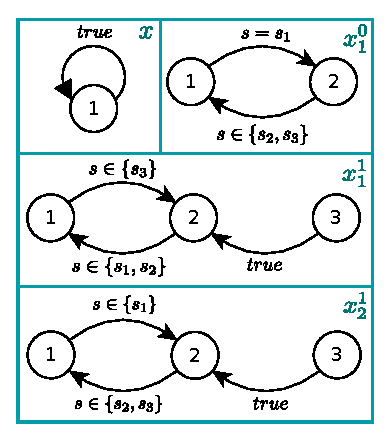
\includegraphics[width=0.7\linewidth]{pic/xupdate2}
%	\caption{ Transition graph of internal variables. Compared to the graph in Figure \ref{fig:eg1}, transition conditions on most edges are different. {\color{purple} What is the difference between the update rule and the transition conditions? I think there is space to put both transition graphs (before and after) on this figure. It would make it easier to see what changed.}}
%	\label{fig:xupdate2}
%\end{figure}

Let the system start from $ s_1 $ and initialize internal variables as $ (1,1,1,1) $. Only one trajectory is available under control of $\widehat{\mathcal{C}} $, i.e. $ s_1,s_2,s_3,s_2,s_1,...$, where the sequence of actions is $ b,f,g,c,... $ according to the controller execution rules in Definition \ref{def:exec}. The trajectory does not visit $ s_4 $, for the system is not able to come back to $ A $ from $ s_4 $ after action $ e $ is removed.

\subsection{Case study: 1D {\color{black} Walking} Robot }

\begin{figure}
	\centering
	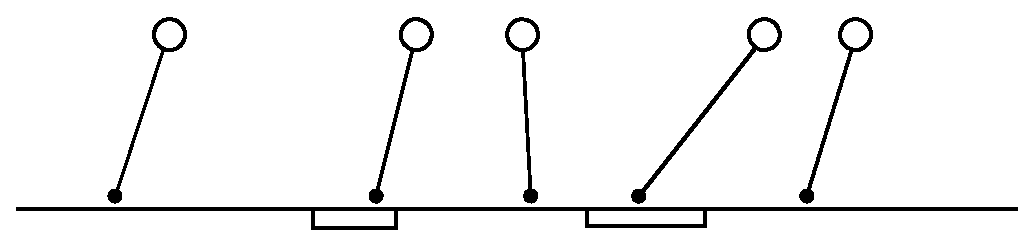
\includegraphics[width=0.5\linewidth]{pic/hop-rob}
	\caption{{\color{black} Simple model of one-legged 1D} robots with point foot {\color{black} walking} on a ground with holes. %{\color{purple} Remark: the linear-inverted pendulum model assumes that the center of mass remains at a fixed height, so this figure can be a bit misleading. But so is the term "walking", so maybe we should just call it "1D walking robot".}
	}	
	\label{fig:hoprob}
\end{figure}

{\color{black} We consider a model of one-legged 1D walking robot moving on a straight line, called the Linear Inverted Pendulum Model (LIPM, see \cite{kajita20013d}). This is a very simplified model of dynamics of a walking robot, but it is used by many algorithms of bipedal walking control (e.g. \cite{englsberger2011bipedal}). It consists in a point-mass robot with a massless leg moving along a line at a constant height above the ground. We do not restrict the extension of the leg nor the velocity of the leg motion (the replacement of the foot is instantaneous). The dynamics of the model are: }
\begin{align}
\begin{bmatrix}
\dot{x}\\
\dot{v}
\end{bmatrix} = \begin{bmatrix}
0 & 1\\
g/h_0 & 0
\end{bmatrix}\begin{bmatrix}
x\\
v
\end{bmatrix}+\begin{bmatrix}
0\\-g/h_0
\end{bmatrix} u \label{eqn: model}
\end{align}
where $x$ is the {\color{black} horizontal position of the} center of mass (CoM) of the robot, $v$ is the velocity of CoM and $ u $ is {\color{black} the horizontal position of the foot.} that the robot foot will step on. 

{\color{black} We consider } the state space $ Q = [-2.5,2.5]\times [-4,4] $ with action space $ U = [-3.5,3.5] $. Discretize $ Q $ and $ U $ uniformly with grid size $ 0.1 $ and $ 0.2 $, and compute the transitions between discretized grids over-approximately  using the method described in \cite{Liu2014,Sun2014}. Finally we get a AFTS $ T $ with states indexed $ [1:4000] $, actions $ [1:35] $ and $ 187594 $ valid transitions, which is the abstraction of the walking robot. 

The specification for the control synthesis is $\Square Q \wedge \Diamond \Square B $,
where $ B=[-2.5,2.5]\times[-2,2] $. It says that the CoM of the robot should always stay within $ [-2.5,2.5] $ with velocity lower than $ 2 $ after finite time from beginning. Given the specification, the winning set and controller are computed via \eqref{win-phi} (taking $ A = Q,B=B , C^1 = Q $).

Now imagine that some holes on the ground are detected, as shown in Figure \ref{fig:hoprob}, where the robot should avoid stepping. Therefore some actions need to be disabled. Once we determine which actions will be affected, we can put them in $ U_d $ and patch the existing controllers for the new action profiles.
\begin{table}
	\centering
	\caption{The execution time of re-synthesis from scratch (row $ 3 $) and patching method (row $ 4 $) under multiple action profiles. The first row is the set of available actions. The second row is the percentage of transitions left after $ U_d $ is disabled.}
	\begin{tabular}{lllllll}
		\hline 
		$ U_d $ & $ [1] $ &$ [1:5] $ & $ [1:10] $ & $ [1:15] $ & $ [1:20] $ & $ [1:25] $ \\ 
		\hline 
		$ \exists $trans & $ 100\% $ & $ 96.57\% $ & $ 81.22\% $ & $ 60.55\% $ & $ 39.67\% $ & $ 19.00\% $\\
		$ t_{syn}(s) $ & $ 244.2 $ & $ 581.2 $ & $ 756.1 $ & $ 532.7 $ & $ 315.1 $ & $ 129.4 $ \\
		$ t_{pat}(s)$ & $ 3.4 $ & $ 12.6 $ & $ 13.4 $ & $ 13.1 $ & $ 11.4 $ & $ 9.9 $ \\ 
		\hline 
	\end{tabular} 
	\label{tab: exper}
\end{table}

\begin{table}
	\centering
	\caption{The average execution time for re-synthesizing from scratch (row $ 2 $), re-synthesizing from the existing winning set, i.e. restrict the state space of the AFTS to be the existing winning set and re-run \eqref{win-phi} (row $ 3 $) and our patching method (row $ 4 $) under random action profiles. The first row is number of unavailable actions ($ \sharp U_d $). For each number, choose 10 random sets of unavailable actions.}
	\begin{tabular}{ccccccc}
		\hline 
		$ \sharp U_d $ & $ 1 $ &$ 5 $ & $ 10 $ & $ 15 $ & $ 20 $ & $ 25 $ \\ 
		\hline 
		$ t_{syn}(s) $ & $ 289.7 $ & $ 281.1 $ & $ 292.8 $ & $ 358.6 $ &  $ 281.5 $ & $ 516.4 $ \\
		$t_{ws} (s)$ & $ 36.2 $ & $ 65.0 $ & $ 108.8 $ & $ 193.9 $ & $ 155.8 $ & $ 371.2 $\\
		$ t_{pat}(s)$ & $ 2.2 $ & $ 2.9 $ & $ 4.2 $ & $ 5.8 $ & $ 7.7 $ & $ 13.9 $ \\ 
		\hline 
	\end{tabular} 
	\label{tab: exper2}
\end{table}

\begin{figure*}
	\centering
	\begin{subfigure}[b]{0.25\textwidth}
		\centering
		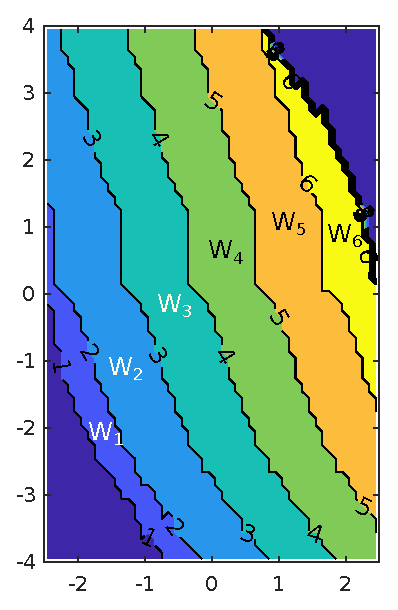
\includegraphics[width=0.8\textwidth]{pic/win-set}
		\caption{winning set}
		\label{fig:winset}
	\end{subfigure}
	%add desired spacing between images, e. g. ~, \quad, \qquad, \hfill etc. 
	%(or a blank line to force the subfigure onto a new line)
	\begin{subfigure}[b]{0.25\textwidth}
		\centering
		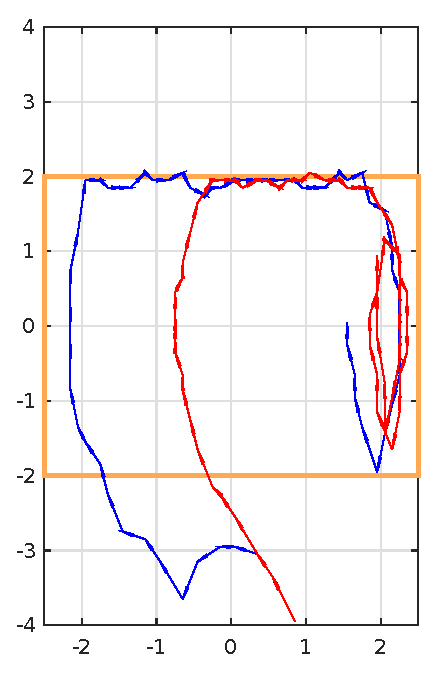
\includegraphics[width=0.8\textwidth]{pic/traj}
		\caption{trajectories}
		\label{fig:traj}
	\end{subfigure}
	%add desired spacing between images, e. g. ~, \quad, \qquad, \hfill etc. 
	%(or a blank line to force the subfigure onto a new line)
	\begin{subfigure}[b]{0.25\textwidth}
		
		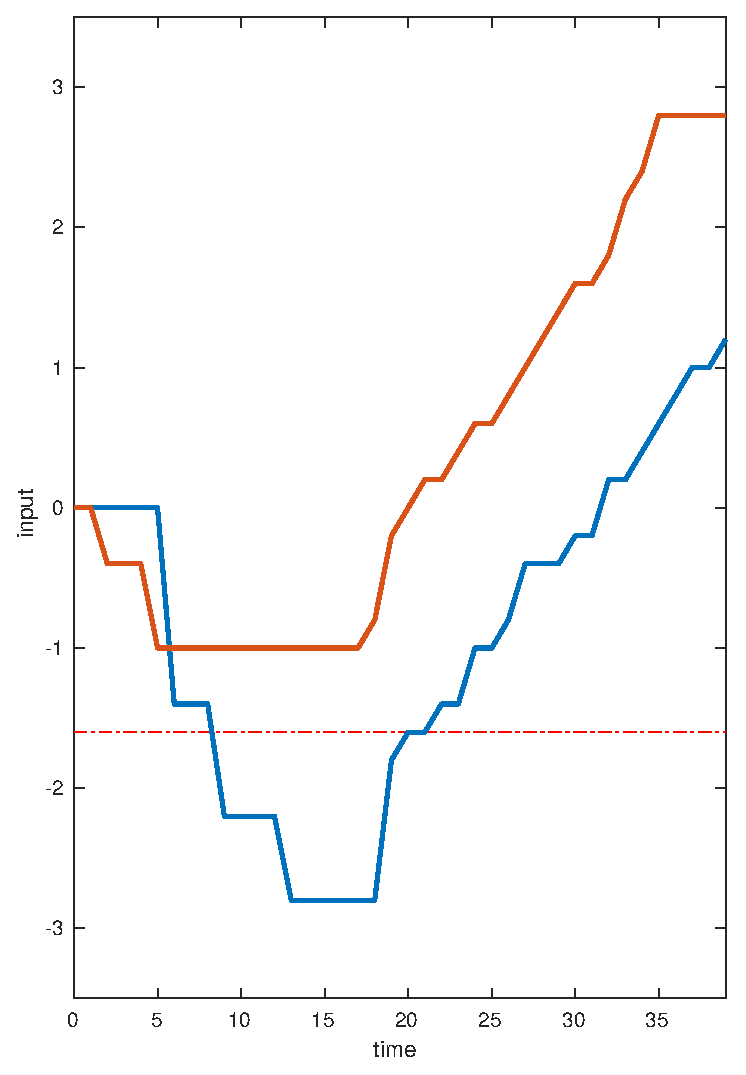
\includegraphics[width=0.85\textwidth]{pic/input}
		\caption{inputs}
		\label{fig:input}
	\end{subfigure}
	\caption{(a) Six regions with different colors are labeled as $ W_1,W_2,...,W6 $. The winning sets under action profiles $U_d = [1], [1:5],[1:10],...,[1:25]$ are the regions corresponding to $ \bigcup_{i=1}^6 W_i,\ \bigcup_{i=2}^6 W_i,\bigcup_{i=3}^6 W_i,...,\ W_6 $ respectively. (b) Trajectories with initial state $ (0.85,-3.95) $ under $ U_d = \emptyset $ (blue) and $[1:10] $ (red). The region inside orange box is the target set $ B $. (c) Inputs over time under $ U_d = \emptyset $ (blue) and $ [1:10] $ (red) for trajectories in (b). The red dash-point line indicates value corresponding to the input indexed by $ u = 10 $.} %{\color{purple} (a) is a bit hard to understand: we  see only disjoint regions on the image but the winning sets are decreasing in size. Maybe say that the winning set $i$ is the union of the $i$ first regions on the graph. (and redefine them accordingly)}
\end{figure*}

The experiment environment is MATLAB R2017a with CPU Intel Core  i7-6820 HQ.

We choose unavailable actions $ U_d= [1],[1:5],...,[1:25] $ for the {\color{black} walking} robot abstraction and compute the controllers via fixed-point operator \eqref{win-phi} and the patching operator \eqref{patch-final} respectively.  The experiment results in Table \ref{tab: exper} make a comparison between the time of synthesizing from scratch ($ t_{syn} $) with the time of patching existing controllers ($ t_{pat} $), which shows that our patching methods can shorten the synthesis time significantly. Figure \ref{fig:winset} shows the winning sets for each $ U_d $, which shrink to the right part in the state space as $ U_d $ (region of holes) grows.

To further show the time efficiency, we randomly choose $ U_d $ with size $n = 1,5,...,25 $. {\color{black}By Theorem \ref{thm: 1}, the winning set after $ U_d $ is removed is contained by the existing one, so we can restrict the state space for the AFTS $ T $ to be the existing winning set and synthesize over this new abstraction via \eqref{win-phi}. Theoretically it saves computation cost, for the new AFTS is smaller. We call it naive warm-starting method. Table \ref{tab: exper2} compares the average time used by naive warm-starting (row $ 3 $) with our patching method (row $ 4 $) and re-synthesizing from scratch (row $ 2 $) for each $ n $.} The time for our patching algorithm is up to $ 3\% $ of the time for re-synthesizing and up to $ 6\% $ of the time for naive warm-starting  on average.

Finally, to show that formal guarantees are satisfied after patching, simulation are run for controllers before and after patching for $ U_d =[1:10]$. The initial state is $ s_0=34 $. Figure \ref{fig:traj} and \ref{fig:input} show the trajectories and the inputs used within $ 60 $ time steps. Both trajectories go into our target region $ B $, indicated by the orange box. The outputs from patched controller is always above the dash line where $ u=10 $, due to the unavailability of actions $[1:10] $.

For practical applications in robot control, if we have the controller for the case that no constraints exists and know all the possible profiles of actions (all the possible constraints on the surface) for a known environment, the patching algorithm can generate the corresponding controllers for those action profiles very quickly. 

\section{CONCLUSION}
In this paper, we proposed an implementation (data structure) for a controller synthesized by fixed-point based control synthesis techniques in \cite{Nilsson2017}. For an existing controller with such a structure, a patching algorithm was developed to modify it for the case that some actions in the original problem setting become unavailable. Furthermore we proved that the winning set resulting from our patching algorithm was exactly the same as the winning set resulting from synthesizing a new controller from scratch. 

We illustrated the efficiency of our method on a example of walking robot. The controller was synthesized for the robot described by a Linear Inverted Pendulum Model with hole constraints on the surface. We first synthesized a controller for a smooth surface without holes, and then patched it using our method for the cases that holes existed. Under the same specification, the time used by our method was only $ 1.4\%-7\% $ of the time used for synthesis from scratch and less than $ 3\% $ on average. 

As future work, it would be interesting to consider cases where the modified action set is not a strict subset of the original action set.  

%It is worth noting that it is possible to construct worst-case examples when the patching method does not provide any speed-ups.  


%{\color{purple} Maybe mention that since in some cases a small change of the action set results in a completely different strategy, we expect that in the worst case, our warm-start method does not bring any speed-up. This is similar to classical warm-up techniques in control: there is no guarantee on the speed-up. And then mention that in future work, although we know that getting formal guarantees on a speed-up in average would be hard (since it highly depends on the type of problem), we wish to conduct a finer study of how much speed-up we can expect to achieve with the proposed warm-up, for instance by studying its effect on "random systems and random specifications}

%The current work is to apply this method on the control synthesis of walking robot on a 2D space. If we force the robot to move in 1D and find a finite set of profiles, this method is able to speed up our synthesis process. Besides, it would be interesting to extend this method for the cases that the specification in \eqref{phi} changes or a set of transitions instead of actions in an AFTS is removed. There is a possibility to do these extension as long as Theorem 1 holds.

\iffalse
\section{Appendix}
\textbf{Proof of \eqref{patch-inv}}:

\emph{Proof:}
	Assume that $ Y_t $ and $ \mathcal{C}_t $ are the winning set and controller resulting from $ \text{Inv}_{\exists}^{D,G} (\widehat{Z}) $. Here we're going to prove that $ Y_t=\widehat{Y}$. Once we have $ Y_t=\widehat{Y}$, it is easy to check that $ A(\mathcal{C}_t) = A(\widehat{\mathcal{C}}) $.
	
	By \eqref{win-inv}, the winning set $ Y $ of $ \text{Inv}_{\exists}^{D,G} (Z) $ is the largest subset of $ (G\cap B) - Z  $ satisfying the convergence condition w.r.t $ Z $, i.e. $ Y \subseteq Pre^{T,D}_{\exists, \forall}(Y\cup Z) $, so is $ Y_t $ w.r.t. $ \widehat{Z} $.
	
	We want to show that $ \widehat{Y} = Y_t$: First, show $ Y_t \subseteq Y_0 $ for $ Y_0 $ in \eqref{patch-inv}. Due to $ Y_t \subseteq G\cap B-\widehat{Z} \subseteq (G\cap B -Z)\cup \Delta Z $, we have $ Y_t\cap (G\cap B-Z)\subseteq Y_t $ and $ Y_t\cup \widehat{Z} \subseteq Y_t\cap (G\cap B-Z)\cup Z$. Then $ Pre^{T,D}_{\exists,\forall}(Y_t\cup \widehat{Z}) \subseteq Pre^{T,D}_{\exists,\forall}(Y_t\cap (G\cap B-Z)\cup Z)$. For $ Y_t \subseteq Pre^{T,D}_{\exists,\forall}(Y_t\cup \widehat{Z})$, we have $ Y_t\cap (G\cap B-Z)\subseteq Pre^{T,D}_{\exists,\forall}(Y_t\cap (G\cap B-Z)\cup Z) $. Therefore $ V= Y_t \cap (G\cap B -Z) $ is one subset of $ G\cap B -Z $ satisfying the convergence condition over $ Z $. For $ V_1 $ and $ V_2 $, two subsets of $ G\cap B-Z $ satisfying convergence condition, $ V_1\cup V_2 $ also satisfies this condition, for $ V_1\cup V_2\subseteq \text{Pre}_{\exists,\forall}(V_1\cup Z)\cup \text{Pre}_{\exists,\forall}(V_2\cup Z)\subseteq \text{Pre}_{\exists,\forall}(V_1\cup V_2\cup Z) $. This implies that $ V \subseteq W_{\text{Inv}} $ (otherwise, $ W_{\text{Inv}} $ could be $ W_{\text{Inv}}\cup V $, since $ W_{\text{Inv}} $ is the largest subset of $ G\cap B-Z $ satisfying the convergence condition over $ Z $.) So $ Y_t = V\cup Y_t\cap \Delta Z \subseteq W_{\text{Inv}}\cup (\Delta Z \cap G\cap B) = Y_0$. 
	
	Next, we want to show that $ Y_t \subseteq Y_{\infty} $. It's equivalent to show that $ \Delta Y_k\cap Y_t = \emptyset $, since $ Y_t\subseteq Y_0 $ and $ Y_k = Y_0 - \bigcup_{i\in \{1,2,...,k\}} \Delta Y_k$. Obviously $ \Delta Y_0\cap (Y_t\cup \widehat{Z}) = \emptyset $. Assume that $ \Delta Y_k \cap (Y_t\cup \widehat{Z}) = \emptyset $, then $ \text{Pre}_{\exists,\forall}^{T,D} (Y_t\cup \widehat{Z}) \cap \text{Pre}_{\forall, \exists}^{T_{\text{Inv}}^k,D}(\Delta Y_k) = \emptyset$ by definition of $ Pre $ in \eqref{eqn:pre} and the fact that $ \rightarrow_{T_{\text{Inv}}^k}\subseteq \rightarrow_{T} $. For $ Y_t \subseteq \text{Pre}_{\exists,\forall}^{T,D} (Y_t\cup \widehat{Z}) $ and $ \Delta Y_{k+1} = \text{Pre}_{\forall, \exists}^{T_{\text{Inv}}^k,D}(\Delta Y_k) $, $ Y_t\cap \Delta Y_{k+1} = \emptyset $. Hence by induction argument, $ Y_t \cap \Delta Y_k = \emptyset, \forall k $. Thus, $ Y_t\subseteq Y_{\infty} $. 
	
	The last step is to show that $ Y_{\infty} $ satisfies the convergence condition over $ \widehat{Z} $. By definitions of $ T_{\text{Inv}}^k $, $ \Delta Y_{k+1}= Y_k \cap \text{Pre}_{\forall,\exists}^{T, D}(\Delta Y_k)$. Then by the additivity of $ \text{Pre}^{T,D}_{\forall,\exists} $ (i.e. for any $ X_1 $ and $ X_2 $, $ \text{Pre}_{\forall,\exists}^{T,D} (X_1\cup X_2)=\text{Pre}_{\forall,\exists}^{T,D} (X_1)\cup \text{Pre}_{\forall,\exists}^{T,D} (X_2) $), it is easy to check that redefining fourth line in \eqref{patch-inv} by $ \Delta Y_{k+1} = \Delta Y_k \cup (Y_k \cap \text{Pre}_{\forall,\exists}^{T, D}(\Delta Y_k)) $ gives the same result.  By the new definition of $ \Delta Y_k $ and the fact $ Y_k \cap \widehat{Z} = \emptyset $, $ \Delta Y_k = Q-(Y_k\cup \widehat{Z}) $. $ \Delta Y_k $ converges surely since it increases each iteration and is contained by a finite set $ Q $. Once $ \Delta Y_k $ converges, $ Y_k \cap \text{Pre}_{\forall,\exists}^{T, D}(\Delta Y_k)\subseteq \Delta Y_k $. $ Y_k $ and $ \Delta Y_k $ are disjoint, so $ Y_k \cap \text{Pre}_{\forall,\exists}^{T, D}(\Delta Y_k) = \emptyset $, i.e.  $ Y_k \cap \text{Pre}_{\forall,\exists}^{T, D}(Q-(Y_k\cup \widehat{Z})) = \emptyset $. It says that $ \forall s_1 \in Y_k$, not $\forall u\in D, \exists s_2\in Q, (s1,u,s2)\in \rightarrow_{T} $ and $s_2\in (Q-(Y_k\cup \widehat{Z}))$, i.e. $ \forall s_1 \in Y_k, \exists u\in D, \forall s_2 \in Q,  (s_1,u,s_2)\not\in \rightarrow_{T}$ or $ s_2\in (Y_k\cup \widehat{Z})$. That implies that $ Y_k\subseteq \text{Pre}_{\exists,\forall}^{T,D}(Y_k\cup \widehat{Z}) $. Therefore $ Y_{\infty}\subseteq Y_t $ following the same arguments in step one. \QEDB
\fi